\documentclass[twoside]{book}

% Packages required by doxygen
\usepackage{fixltx2e}
\usepackage{calc}
\usepackage{doxygen}
\usepackage[export]{adjustbox} % also loads graphicx
\usepackage{graphicx}
\usepackage[utf8]{inputenc}
\usepackage{makeidx}
\usepackage{multicol}
\usepackage{multirow}
\PassOptionsToPackage{warn}{textcomp}
\usepackage{textcomp}
\usepackage[nointegrals]{wasysym}
\usepackage[table]{xcolor}

% Font selection
\usepackage[T1]{fontenc}
\usepackage[scaled=.90]{helvet}
\usepackage{courier}
\usepackage{amssymb}
\usepackage{sectsty}
\renewcommand{\familydefault}{\sfdefault}
\allsectionsfont{%
  \fontseries{bc}\selectfont%
  \color{darkgray}%
}
\renewcommand{\DoxyLabelFont}{%
  \fontseries{bc}\selectfont%
  \color{darkgray}%
}
\newcommand{\+}{\discretionary{\mbox{\scriptsize$\hookleftarrow$}}{}{}}

% Page & text layout
\usepackage{geometry}
\geometry{%
  a4paper,%
  top=2.5cm,%
  bottom=2.5cm,%
  left=2.5cm,%
  right=2.5cm%
}
\tolerance=750
\hfuzz=15pt
\hbadness=750
\setlength{\emergencystretch}{15pt}
\setlength{\parindent}{0cm}
\setlength{\parskip}{3ex plus 2ex minus 2ex}
\makeatletter
\renewcommand{\paragraph}{%
  \@startsection{paragraph}{4}{0ex}{-1.0ex}{1.0ex}{%
    \normalfont\normalsize\bfseries\SS@parafont%
  }%
}
\renewcommand{\subparagraph}{%
  \@startsection{subparagraph}{5}{0ex}{-1.0ex}{1.0ex}{%
    \normalfont\normalsize\bfseries\SS@subparafont%
  }%
}
\makeatother

% Headers & footers
\usepackage{fancyhdr}
\pagestyle{fancyplain}
\fancyhead[LE]{\fancyplain{}{\bfseries\thepage}}
\fancyhead[CE]{\fancyplain{}{}}
\fancyhead[RE]{\fancyplain{}{\bfseries\leftmark}}
\fancyhead[LO]{\fancyplain{}{\bfseries\rightmark}}
\fancyhead[CO]{\fancyplain{}{}}
\fancyhead[RO]{\fancyplain{}{\bfseries\thepage}}
\fancyfoot[LE]{\fancyplain{}{}}
\fancyfoot[CE]{\fancyplain{}{}}
\fancyfoot[RE]{\fancyplain{}{\bfseries\scriptsize Generated by Doxygen }}
\fancyfoot[LO]{\fancyplain{}{\bfseries\scriptsize Generated by Doxygen }}
\fancyfoot[CO]{\fancyplain{}{}}
\fancyfoot[RO]{\fancyplain{}{}}
\renewcommand{\footrulewidth}{0.4pt}
\renewcommand{\chaptermark}[1]{%
  \markboth{#1}{}%
}
\renewcommand{\sectionmark}[1]{%
  \markright{\thesection\ #1}%
}

% Indices & bibliography
\usepackage{natbib}
\usepackage[titles]{tocloft}
\setcounter{tocdepth}{3}
\setcounter{secnumdepth}{5}
\makeindex

% Hyperlinks (required, but should be loaded last)
\usepackage{ifpdf}
\ifpdf
  \usepackage[pdftex,pagebackref=true]{hyperref}
\else
  \usepackage[ps2pdf,pagebackref=true]{hyperref}
\fi
\hypersetup{%
  colorlinks=true,%
  linkcolor=blue,%
  citecolor=blue,%
  unicode%
}

% Custom commands
\newcommand{\clearemptydoublepage}{%
  \newpage{\pagestyle{empty}\cleardoublepage}%
}

\usepackage{caption}
\captionsetup{labelsep=space,justification=centering,font={bf},singlelinecheck=off,skip=4pt,position=top}

%===== C O N T E N T S =====

\begin{document}

% Titlepage & ToC
\hypersetup{pageanchor=false,
             bookmarksnumbered=true,
             pdfencoding=unicode
            }
\pagenumbering{alph}
\begin{titlepage}
\vspace*{7cm}
\begin{center}%
{\Large E\+S\+Pmanager }\\
\vspace*{1cm}
{\large Generated by Doxygen 1.8.13}\\
\end{center}
\end{titlepage}
\clearemptydoublepage
\pagenumbering{roman}
\tableofcontents
\clearemptydoublepage
\pagenumbering{arabic}
\hypersetup{pageanchor=true}

%--- Begin generated contents ---
\chapter{readme}
\label{md_src__tasker_readme}
\Hypertarget{md_src__tasker_readme}
This is an attempt at a task schedular for E\+S\+P8266. Written in c++.

Most of the complexities are hidden under the hood, it seems to work very well.

\section*{Key features\+:}


\begin{DoxyItemize}
\item Non\+Blocking. The loop is not blocked, as long as you do not call delay() in your functions.
\item Flexible. All tasks are std\+::function calls so can use std\+::bind or lambdas.
\item A\+Sync\+Tasker -\/ Creates a task instance that runs all tasks concurrently, usefull for driving displays whilst checking buttons etc. non premtive multitasking!
\begin{DoxyItemize}
\item This feature has a timeout feature so each loop cycle it will visit each task to see if it needs running. If one task takes more than the timeout then it exits, continuing where it left of next loop. This allows you to maintain say wifi or other tasks as well.
\end{DoxyItemize}
\item Sync\+Tasker -\/ Creates a sequential \hyperlink{class_tasker}{Tasker} that waits for previous event to finish before starting the next.
\begin{DoxyItemize}
\item This is good for running a sequence of events that depend on the previous finishing. This tasker can be set to repeat which will continue to loop around. See Blink example using this.
\end{DoxyItemize}
\item add\+Sub\+Tasker$<$class Tasker\+Type$>$(\+Tasker\+Type tasker) -\/ This function is very powerfull. It creates a new tasker, and adds the required loop functions to the parent tasker, and returns a pointer back to this new \hyperlink{class_tasker}{Tasker}. Available to any \hyperlink{class_tasker}{Tasker} instance. This allows you in any task to spawn a new tasker to run sync, or async along side existing tasks!! all non blocking!
\item Templated Tasks and loop methods, allow you to design your own \hyperlink{class_task}{Task} types and loop methods if required, the basic typedefs are created for you {\ttfamily A\+Sync\+Tasker} and {\ttfamily Sync\+Tasker}. Plans are to implement light weight methods and tasks that don\textquotesingle{}t occupy much R\+AM. So you can develop using the verbose outputs, and switch to lightweight for production.
\end{DoxyItemize}

\subsubsection*{Examples}

Basic 
\begin{DoxyCode}
\textcolor{preprocessor}{#include <\hyperlink{_tasker_8h}{Tasker.h}>}

\hyperlink{class_tasker}{ASyncTasker} tasker; 

\textcolor{keywordtype}{void} setup() \{
  Serial.begin(115200);
  Serial.print(\textcolor{stringliteral}{"\(\backslash\)nBOOTING...."});
    \textcolor{comment}{// prints hello after 10 seconds. }
    tasker.add( [] (\hyperlink{class_task}{Task} & t) \{
        Serial.println(\textcolor{stringliteral}{"hello"}); 
    \}).setTimeout(10000); 
   \textcolor{comment}{// prints hello again after 20 seconds }
    tasker.add( [] (\hyperlink{class_task}{Task} & t) \{
        Serial.println(\textcolor{stringliteral}{"hello again"}); 
    \}).setTimeout(20000);  
Serial.println(\textcolor{stringliteral}{"READY\(\backslash\)n"});
\}

\textcolor{keywordtype}{void} loop() \{
tasker.loop();
\}
\end{DoxyCode}


These two tasks run at the same time. This next example adds two tasks to a Sync\+Tasker, which waits for the first task to run before running the next. Declare {\ttfamily Sync\+Tasker tasker;} instead of {\ttfamily A\+Sync\+Tasker tasker;} then each task will follow the next. \subsubsection*{Tasks}

Tasks are created internally with std\+::unique\+\_\+ptr, they are deleted when they are complete. A reference is returned to the pointer at creation allowing you to set and change parameters, but do not convert to a pointer, as the lifetime of the object is not guarunteed! you have been warned! I may implement a method to check if a task is still running...

Each task callback is called with a reference to the task, so all task properties are changable within the callback. This allows you to test a condition and then change it at run time. eg 
\begin{DoxyCode}
\hyperlink{class_task}{Task} & t = tasker.add( [] (\hyperlink{class_task}{Task} & t) \{
     Serial.println(\textcolor{stringliteral}{"hello again"}); 
     t.setRepeat(\textcolor{keyword}{false}); \textcolor{comment}{//  changes to no repeating, and deletes the task.}
     uint32\_t count = t.count; \textcolor{comment}{// returns the run number. }
     t.setTimeout(1000); \textcolor{comment}{//  change the timout to 1 second from 20 seconds! }
 \}).setTimeout(20000).setRepeat(\textcolor{keyword}{true}); 
\end{DoxyCode}


Tasks can also be named {\ttfamily .set\+Name(const char $\ast$)}, good for debugging as the name will appear in the debug output. \#\#\# Creating subtasks 
\begin{DoxyCode}
auto subtasker = tasker.addSubTasker<SyncTasker>();
\end{DoxyCode}
 This gives you a pointer to the sub tasker, behind the scenes it adds a loop() to the parent tasker, which is automatically deleted when the count of tasks == 0. This is unless you use {\ttfamily auto subtasker = tasker.\+add\+Sub\+Tasker$<$Sync\+Tasker$>$(true)}, which prevents the subtasker from being deleted. Unless you\textquotesingle{}ve set this to true, it is probably safe to assume that the tasker has been deleted and you\textquotesingle{}re accessing a null ptr!

\subsubsection*{Debug out}

Using {\ttfamily tasker.\+debug\+Out(\+Serial);} gives you a list of all the current running tasks, and subtasks. 
\begin{DoxyCode}
*****  Tasker  *****  
Heap: 43320
Tasker: 0x3ffef290 - 4 Tasks Running
    1. 0x3fff0a0c [N][Debug Out] priority 0, timeout = 10000, runcount = 1
    2. Tasker: 0x3fff0a88 - 4 Tasks Running Parent Tasker 0x3ffef290
       └ 1. 0x3fff0b14 [N][SubTask1.1] timeout = 30000, runcount = 0
        └ 2. 0x3fff0b74 [N][SubTask1.2] timeout = 30000, runcount = 0
         └ 3. 0x3fff0bd4 [N][SubTask1.3] timeout = 30000, runcount = 0
          └ 4. 0x3fff0c3c [N][SubTask1.4] timeout = 30000, runcount = 0
    3. Tasker: 0x3fff0cb8 - 1 Tasks Running Parent Tasker 0x3ffef290
        └ 1. Tasker: 0x3fff0e88 - 1 Tasks Running Parent Tasker 0x3fff0cb8
            1. Tasker: 0x3fff1328 - 20 Tasks Running Parent Tasker 0x3fff0e88
               └ 1. 0x3fff13c4 [N][supernested] timeout = 10000, runcount = 0
                └ 2. 0x3fff140c [N][supernested] timeout = 10000, runcount = 0
                 └ 3. 0x3fff1474 [N][supernested] timeout = 10000, runcount = 0
*****   END   *****
\end{DoxyCode}
 Tasks run async just appear as numbers, tasks run sync and depend on the previous finishing have └ and are indented. The memory location of all taskers and tasks is given to help debugging.

\subsubsection*{Other}


\begin{DoxyItemize}
\item There are plans for a priority approach but it has not been implemented yet... watch this space.
\item I also plan to write lightweight less R\+AM hungry versions. 
\end{DoxyItemize}
\chapter{Hierarchical Index}
\section{Class Hierarchy}
This inheritance list is sorted roughly, but not completely, alphabetically\+:\begin{DoxyCompactList}
\item \contentsline{section}{E\+S\+P\+M\+AN\+:\+:settings\+\_\+t\+:\+:A\+P\+\_\+t}{\pageref{struct_e_s_p_m_a_n_1_1settings__t_1_1_a_p__t}}{}
\item \contentsline{section}{base\+Methods}{\pageref{classbase_methods}}{}
\begin{DoxyCompactList}
\item \contentsline{section}{A\+Sync$<$ T $>$}{\pageref{class_a_sync}}{}
\item \contentsline{section}{A\+Sync$<$ Task $>$}{\pageref{class_a_sync}}{}
\begin{DoxyCompactList}
\item \contentsline{section}{Tasker$<$ Task, A\+Sync$<$ Task $>$ $>$}{\pageref{class_tasker}}{}
\end{DoxyCompactList}
\item \contentsline{section}{Sync$<$ T $>$}{\pageref{class_sync}}{}
\end{DoxyCompactList}
\item \contentsline{section}{E\+S\+Pdevice\+Finder}{\pageref{class_e_s_pdevice_finder}}{}
\item \contentsline{section}{E\+S\+Pmanager}{\pageref{class_e_s_pmanager}}{}
\item \contentsline{section}{E\+S\+P\+M\+AN\+:\+:settings\+\_\+t\+:\+:G\+E\+N\+\_\+t}{\pageref{struct_e_s_p_m_a_n_1_1settings__t_1_1_g_e_n__t}}{}
\item \contentsline{section}{E\+S\+P\+M\+AN\+:\+:J\+S\+O\+Npackage}{\pageref{class_e_s_p_m_a_n_1_1_j_s_o_npackage}}{}
\item \contentsline{section}{E\+S\+P\+M\+AN\+:\+:my\+String}{\pageref{class_e_s_p_m_a_n_1_1my_string}}{}
\begin{DoxyCompactList}
\item \contentsline{section}{E\+S\+P\+M\+AN\+:\+:my\+Stringf}{\pageref{class_e_s_p_m_a_n_1_1my_stringf}}{}
\item \contentsline{section}{E\+S\+P\+M\+AN\+:\+:my\+Stringf\+\_\+P}{\pageref{class_e_s_p_m_a_n_1_1my_stringf___p}}{}
\end{DoxyCompactList}
\item \contentsline{section}{E\+S\+P\+M\+AN\+:\+:password\+\_\+t}{\pageref{struct_e_s_p_m_a_n_1_1password__t}}{}
\item \contentsline{section}{E\+S\+P\+M\+AN\+:\+:settings\+\_\+t}{\pageref{struct_e_s_p_m_a_n_1_1settings__t}}{}
\item \contentsline{section}{Simple\+Task}{\pageref{class_simple_task}}{}
\item \contentsline{section}{E\+S\+P\+M\+AN\+:\+:settings\+\_\+t\+:\+:S\+T\+A\+\_\+t}{\pageref{struct_e_s_p_m_a_n_1_1settings__t_1_1_s_t_a__t}}{}
\item Stream\begin{DoxyCompactList}
\item \contentsline{section}{Flash\+Writer}{\pageref{class_flash_writer}}{}
\end{DoxyCompactList}
\item \contentsline{section}{Sys\+Log}{\pageref{class_sys_log}}{}
\item \contentsline{section}{Task}{\pageref{class_task}}{}
\item \contentsline{section}{Tasker\+Base}{\pageref{class_tasker_base}}{}
\begin{DoxyCompactList}
\item \contentsline{section}{Tasker$<$ Task\+Type, Loop\+Method $>$}{\pageref{class_tasker}}{}
\item \contentsline{section}{Tasker$<$ Task, A\+Sync$<$ Task $>$ $>$}{\pageref{class_tasker}}{}
\end{DoxyCompactList}
\item \contentsline{section}{E\+S\+Pdevice\+Finder\+:\+:U\+D\+P\+\_\+item}{\pageref{struct_e_s_pdevice_finder_1_1_u_d_p__item}}{}
\item Loop\+Method\begin{DoxyCompactList}
\item \contentsline{section}{Tasker$<$ Task\+Type, Loop\+Method $>$}{\pageref{class_tasker}}{}
\end{DoxyCompactList}
\end{DoxyCompactList}

\chapter{Class Index}
\section{Class List}
Here are the classes, structs, unions and interfaces with brief descriptions\+:\begin{DoxyCompactList}
\item\contentsline{section}{\hyperlink{struct_e_s_p_m_a_n_1_1settings__t_1_1_a_p__t}{E\+S\+P\+M\+A\+N\+::settings\+\_\+t\+::\+A\+P\+\_\+t} }{\pageref{struct_e_s_p_m_a_n_1_1settings__t_1_1_a_p__t}}{}
\item\contentsline{section}{\hyperlink{class_a_sync}{A\+Sync$<$ T $>$} }{\pageref{class_a_sync}}{}
\item\contentsline{section}{\hyperlink{classbase_methods}{base\+Methods} }{\pageref{classbase_methods}}{}
\item\contentsline{section}{\hyperlink{class_e_s_pdevice_finder}{E\+S\+Pdevice\+Finder} }{\pageref{class_e_s_pdevice_finder}}{}
\item\contentsline{section}{\hyperlink{class_e_s_pmanager}{E\+S\+Pmanager} }{\pageref{class_e_s_pmanager}}{}
\item\contentsline{section}{\hyperlink{class_flash_writer}{Flash\+Writer} }{\pageref{class_flash_writer}}{}
\item\contentsline{section}{\hyperlink{struct_e_s_p_m_a_n_1_1settings__t_1_1_g_e_n__t}{E\+S\+P\+M\+A\+N\+::settings\+\_\+t\+::\+G\+E\+N\+\_\+t} }{\pageref{struct_e_s_p_m_a_n_1_1settings__t_1_1_g_e_n__t}}{}
\item\contentsline{section}{\hyperlink{class_e_s_p_m_a_n_1_1_j_s_o_npackage}{E\+S\+P\+M\+A\+N\+::\+J\+S\+O\+Npackage} }{\pageref{class_e_s_p_m_a_n_1_1_j_s_o_npackage}}{}
\item\contentsline{section}{\hyperlink{class_e_s_p_m_a_n_1_1my_string}{E\+S\+P\+M\+A\+N\+::my\+String} }{\pageref{class_e_s_p_m_a_n_1_1my_string}}{}
\item\contentsline{section}{\hyperlink{class_e_s_p_m_a_n_1_1my_stringf}{E\+S\+P\+M\+A\+N\+::my\+Stringf} }{\pageref{class_e_s_p_m_a_n_1_1my_stringf}}{}
\item\contentsline{section}{\hyperlink{class_e_s_p_m_a_n_1_1my_stringf___p}{E\+S\+P\+M\+A\+N\+::my\+Stringf\+\_\+P} }{\pageref{class_e_s_p_m_a_n_1_1my_stringf___p}}{}
\item\contentsline{section}{\hyperlink{struct_e_s_p_m_a_n_1_1password__t}{E\+S\+P\+M\+A\+N\+::password\+\_\+t} }{\pageref{struct_e_s_p_m_a_n_1_1password__t}}{}
\item\contentsline{section}{\hyperlink{struct_e_s_p_m_a_n_1_1settings__t}{E\+S\+P\+M\+A\+N\+::settings\+\_\+t} }{\pageref{struct_e_s_p_m_a_n_1_1settings__t}}{}
\item\contentsline{section}{\hyperlink{class_simple_task}{Simple\+Task} }{\pageref{class_simple_task}}{}
\item\contentsline{section}{\hyperlink{struct_e_s_p_m_a_n_1_1settings__t_1_1_s_t_a__t}{E\+S\+P\+M\+A\+N\+::settings\+\_\+t\+::\+S\+T\+A\+\_\+t} }{\pageref{struct_e_s_p_m_a_n_1_1settings__t_1_1_s_t_a__t}}{}
\item\contentsline{section}{\hyperlink{class_sync}{Sync$<$ T $>$} }{\pageref{class_sync}}{}
\item\contentsline{section}{\hyperlink{class_sys_log}{Sys\+Log} }{\pageref{class_sys_log}}{}
\item\contentsline{section}{\hyperlink{class_task}{Task} }{\pageref{class_task}}{}
\item\contentsline{section}{\hyperlink{class_tasker}{Tasker$<$ Task\+Type, Loop\+Method $>$} }{\pageref{class_tasker}}{}
\item\contentsline{section}{\hyperlink{class_tasker_base}{Tasker\+Base} }{\pageref{class_tasker_base}}{}
\item\contentsline{section}{\hyperlink{struct_e_s_pdevice_finder_1_1_u_d_p__item}{E\+S\+Pdevice\+Finder\+::\+U\+D\+P\+\_\+item} }{\pageref{struct_e_s_pdevice_finder_1_1_u_d_p__item}}{}
\end{DoxyCompactList}

\chapter{File Index}
\section{File List}
Here is a list of all documented files with brief descriptions\+:\begin{DoxyCompactList}
\item\contentsline{section}{src/\hyperlink{_e_s_p_m_a_n_8cpp}{E\+S\+P\+M\+A\+N.\+cpp} \\*E\+S\+P\+M\+AN file }{\pageref{_e_s_p_m_a_n_8cpp}}{}
\item\contentsline{section}{src/\hyperlink{_e_s_p_m_a_n_8h}{E\+S\+P\+M\+A\+N.\+h} \\*E\+S\+P\+M\+AN file }{\pageref{_e_s_p_m_a_n_8h}}{}
\item\contentsline{section}{src/\hyperlink{_e_s_pmanager_8cpp}{E\+S\+Pmanager.\+cpp} \\*\hyperlink{class_e_s_pmanager}{E\+S\+Pmanager} file }{\pageref{_e_s_pmanager_8cpp}}{}
\item\contentsline{section}{src/\hyperlink{_e_s_pmanager_8h}{E\+S\+Pmanager.\+h} \\*\hyperlink{class_e_s_pmanager}{E\+S\+Pmanager} file }{\pageref{_e_s_pmanager_8h}}{}
\item\contentsline{section}{src/\hyperlink{_e_s_pman_sys_log_8cpp}{E\+S\+Pman\+Sys\+Log.\+cpp} \\*Syslog implementation file }{\pageref{_e_s_pman_sys_log_8cpp}}{}
\item\contentsline{section}{src/\hyperlink{_e_s_pman_sys_log_8h}{E\+S\+Pman\+Sys\+Log.\+h} \\*\hyperlink{class_e_s_pmanager}{E\+S\+Pmanager} file }{\pageref{_e_s_pman_sys_log_8h}}{}
\item\contentsline{section}{src/{\bfseries favicon.\+h} }{\pageref{favicon_8h}}{}
\item\contentsline{section}{src/\hyperlink{_flash_writer_8cpp}{Flash\+Writer.\+cpp} \\*Flashwriter file }{\pageref{_flash_writer_8cpp}}{}
\item\contentsline{section}{src/\hyperlink{_flash_writer_8h}{Flash\+Writer.\+h} \\*\hyperlink{class_e_s_pmanager}{E\+S\+Pmanager} file }{\pageref{_flash_writer_8h}}{}
\item\contentsline{section}{src/\hyperlink{_save_stack_8h}{Save\+Stack.\+h} \\*Save Stack file }{\pageref{_save_stack_8h}}{}
\item\contentsline{section}{src/\+E\+S\+Pdevice\+Finder/src/{\bfseries E\+S\+Pdevice\+Finder.\+h} }{\pageref{_e_s_pdevice_finder_8h}}{}
\item\contentsline{section}{src/\+Tasker/src/\hyperlink{_task_8h}{Task.\+h} \\*\hyperlink{class_task}{Task} file }{\pageref{_task_8h}}{}
\item\contentsline{section}{src/\+Tasker/src/\hyperlink{_tasker_8h}{Tasker.\+h} \\*\hyperlink{class_tasker}{Tasker} file }{\pageref{_tasker_8h}}{}
\item\contentsline{section}{src/\+Tasker/src/\hyperlink{_tasker_class_8h}{Tasker\+Class.\+h} \\*\hyperlink{class_tasker}{Tasker} file }{\pageref{_tasker_class_8h}}{}
\item\contentsline{section}{src/\+Tasker/src/\hyperlink{_task_methods_8h}{Task\+Methods.\+h} \\*Loop Methods for \hyperlink{class_tasker}{Tasker} Type file }{\pageref{_task_methods_8h}}{}
\end{DoxyCompactList}

\chapter{Class Documentation}
\hypertarget{struct_e_s_p_m_a_n_1_1settings__t_1_1_a_p__t}{}\section{E\+S\+P\+M\+AN\+:\+:settings\+\_\+t\+:\+:A\+P\+\_\+t Struct Reference}
\label{struct_e_s_p_m_a_n_1_1settings__t_1_1_a_p__t}\index{E\+S\+P\+M\+A\+N\+::settings\+\_\+t\+::\+A\+P\+\_\+t@{E\+S\+P\+M\+A\+N\+::settings\+\_\+t\+::\+A\+P\+\_\+t}}
\subsection*{Public Attributes}
\begin{DoxyCompactItemize}
\item 
\mbox{\Hypertarget{struct_e_s_p_m_a_n_1_1settings__t_1_1_a_p__t_af33864067824cd2b70b570d978b3f839}\label{struct_e_s_p_m_a_n_1_1settings__t_1_1_a_p__t_af33864067824cd2b70b570d978b3f839}} 
bool {\bfseries enabled} \{false\}
\item 
\mbox{\Hypertarget{struct_e_s_p_m_a_n_1_1settings__t_1_1_a_p__t_a4abf044830a12f4caeb89fadd484af9a}\label{struct_e_s_p_m_a_n_1_1settings__t_1_1_a_p__t_a4abf044830a12f4caeb89fadd484af9a}} 
bool {\bfseries has\+Config} \{false\}
\item 
\mbox{\Hypertarget{struct_e_s_p_m_a_n_1_1settings__t_1_1_a_p__t_ab8d0cfa8c4f57cacad796779b3f84ff0}\label{struct_e_s_p_m_a_n_1_1settings__t_1_1_a_p__t_ab8d0cfa8c4f57cacad796779b3f84ff0}} 
bool {\bfseries has\+M\+AC} \{false\}
\item 
\mbox{\Hypertarget{struct_e_s_p_m_a_n_1_1settings__t_1_1_a_p__t_a207de9b69255b23b0963e91d5cd73098}\label{struct_e_s_p_m_a_n_1_1settings__t_1_1_a_p__t_a207de9b69255b23b0963e91d5cd73098}} 
\hyperlink{class_e_s_p_m_a_n_1_1my_string}{my\+String} {\bfseries ssid}
\item 
\mbox{\Hypertarget{struct_e_s_p_m_a_n_1_1settings__t_1_1_a_p__t_a4f8c96737f9aa05c61324eed261ef133}\label{struct_e_s_p_m_a_n_1_1settings__t_1_1_a_p__t_a4f8c96737f9aa05c61324eed261ef133}} 
\hyperlink{class_e_s_p_m_a_n_1_1my_string}{my\+String} {\bfseries pass}
\item 
\mbox{\Hypertarget{struct_e_s_p_m_a_n_1_1settings__t_1_1_a_p__t_a5889ccecc4c8bafa7c2f85ce533c95e3}\label{struct_e_s_p_m_a_n_1_1settings__t_1_1_a_p__t_a5889ccecc4c8bafa7c2f85ce533c95e3}} 
I\+P\+Address {\bfseries IP}
\item 
\mbox{\Hypertarget{struct_e_s_p_m_a_n_1_1settings__t_1_1_a_p__t_a476475a40c3c67af6a67e374b09f7778}\label{struct_e_s_p_m_a_n_1_1settings__t_1_1_a_p__t_a476475a40c3c67af6a67e374b09f7778}} 
I\+P\+Address {\bfseries GW}
\item 
\mbox{\Hypertarget{struct_e_s_p_m_a_n_1_1settings__t_1_1_a_p__t_ab700a89554f05a4065771146e00ff046}\label{struct_e_s_p_m_a_n_1_1settings__t_1_1_a_p__t_ab700a89554f05a4065771146e00ff046}} 
I\+P\+Address {\bfseries SN}
\item 
\mbox{\Hypertarget{struct_e_s_p_m_a_n_1_1settings__t_1_1_a_p__t_a5c57f0c7577a7eab7c5c2a930ab06c78}\label{struct_e_s_p_m_a_n_1_1settings__t_1_1_a_p__t_a5c57f0c7577a7eab7c5c2a930ab06c78}} 
uint8\+\_\+t {\bfseries M\+AC} \mbox{[}6\mbox{]} = \{\textquotesingle{}\textbackslash{}0\textquotesingle{}\}
\item 
\mbox{\Hypertarget{struct_e_s_p_m_a_n_1_1settings__t_1_1_a_p__t_a367ab9d8bfc49892fbd4a49dbab137fe}\label{struct_e_s_p_m_a_n_1_1settings__t_1_1_a_p__t_a367ab9d8bfc49892fbd4a49dbab137fe}} 
bool {\bfseries visible} \{true\}
\item 
\mbox{\Hypertarget{struct_e_s_p_m_a_n_1_1settings__t_1_1_a_p__t_a68b5bf8779a313d5989a70e795299ca2}\label{struct_e_s_p_m_a_n_1_1settings__t_1_1_a_p__t_a68b5bf8779a313d5989a70e795299ca2}} 
uint8\+\_\+t {\bfseries channel} \{1\}
\end{DoxyCompactItemize}


The documentation for this struct was generated from the following file\+:\begin{DoxyCompactItemize}
\item 
src/\hyperlink{_e_s_p_m_a_n_8h}{E\+S\+P\+M\+A\+N.\+h}\end{DoxyCompactItemize}

\hypertarget{class_a_sync}{}\section{A\+Sync$<$ T $>$ Class Template Reference}
\label{class_a_sync}\index{A\+Sync$<$ T $>$@{A\+Sync$<$ T $>$}}
Inheritance diagram for A\+Sync$<$ T $>$\+:\begin{figure}[H]
\begin{center}
\leavevmode
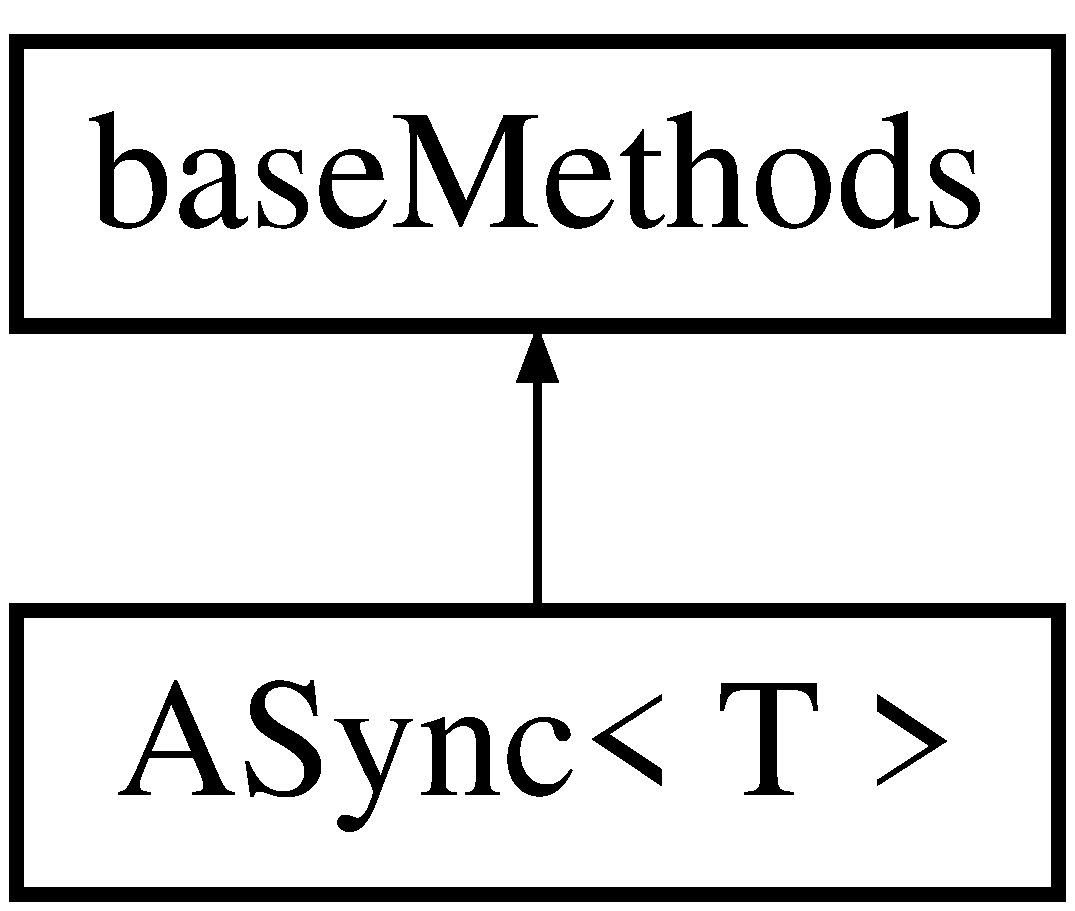
\includegraphics[height=2.000000cm]{class_a_sync}
\end{center}
\end{figure}
\subsection*{Public Types}
\begin{DoxyCompactItemize}
\item 
\mbox{\Hypertarget{class_a_sync_ad027c26566d61730f6d924723063a8f8}\label{class_a_sync_ad027c26566d61730f6d924723063a8f8}} 
typedef std\+::unique\+\_\+ptr$<$ T $>$ {\bfseries task\+Storage\+\_\+t}
\item 
\mbox{\Hypertarget{class_a_sync_ae803791a9b07ed69df45788faf2b1056}\label{class_a_sync_ae803791a9b07ed69df45788faf2b1056}} 
typedef \hyperlink{class_tasker_base}{Tasker\+Base} $\ast$ {\bfseries sub\+Task\+Storage\+\_\+t}
\item 
\mbox{\Hypertarget{class_a_sync_aaf7916c6d943c8411ec46925d90a8980}\label{class_a_sync_aaf7916c6d943c8411ec46925d90a8980}} 
typedef std\+::pair$<$ task\+Storage\+\_\+t, \hyperlink{class_tasker_base}{sub\+Task\+Storage\+\_\+t} $>$ {\bfseries task\+Pair\+Storage\+\_\+t}
\item 
\mbox{\Hypertarget{class_a_sync_a29faf063ec9cf599ff7972bd568c8bd6}\label{class_a_sync_a29faf063ec9cf599ff7972bd568c8bd6}} 
typedef std\+::list$<$ task\+Pair\+Storage\+\_\+t $>$ {\bfseries task\+List\+\_\+t}
\item 
\mbox{\Hypertarget{class_a_sync_acf02876cf46228842bf522e2472047fc}\label{class_a_sync_acf02876cf46228842bf522e2472047fc}} 
typedef std\+::function$<$ void(void)$>$ {\bfseries Empty\+Cb\+\_\+t}
\item 
\mbox{\Hypertarget{class_a_sync_a89b833f9d18c705542e44c0cf06bd755}\label{class_a_sync_a89b833f9d18c705542e44c0cf06bd755}} 
typedef std\+::function$<$ void(T \&)$>$ {\bfseries tasker\+Cb\+\_\+t}
\end{DoxyCompactItemize}
\subsection*{Public Member Functions}
\begin{DoxyCompactItemize}
\item 
\mbox{\Hypertarget{class_a_sync_ad586983c3b5453864c12d37d5d6b7fad}\label{class_a_sync_ad586983c3b5453864c12d37d5d6b7fad}} 
void {\bfseries loop} ()
\item 
\mbox{\Hypertarget{class_a_sync_a6333015d654162322cfd09f13fe7ba44}\label{class_a_sync_a6333015d654162322cfd09f13fe7ba44}} 
void {\bfseries set\+Priority} (uint8\+\_\+t priority)
\item 
\mbox{\Hypertarget{class_a_sync_a5a427b4d80c9483aba739dfe11e85aef}\label{class_a_sync_a5a427b4d80c9483aba739dfe11e85aef}} 
uint8\+\_\+t {\bfseries get\+Priority} ()
\item 
\mbox{\Hypertarget{class_a_sync_a09aeb7ecadb4e7ec34c20565914ad112}\label{class_a_sync_a09aeb7ecadb4e7ec34c20565914ad112}} 
void {\bfseries set\+Max\+Waitus} (uint32\+\_\+t wait)
\item 
\mbox{\Hypertarget{class_a_sync_a340dacc4205e0386ee5c5e38b0f789a4}\label{class_a_sync_a340dacc4205e0386ee5c5e38b0f789a4}} 
void {\bfseries dump\+Task} (T \&t, Stream \&stream, uint \&position, uint index)
\item 
\mbox{\Hypertarget{class_a_sync_a00ce789e4369a80307d8f4b010fe3fc9}\label{class_a_sync_a00ce789e4369a80307d8f4b010fe3fc9}} 
void {\bfseries printprechar} (Stream \&stream)
\end{DoxyCompactItemize}
\subsection*{Public Attributes}
\begin{DoxyCompactItemize}
\item 
\mbox{\Hypertarget{class_a_sync_ac5922c45fbedb75745fc665619d8ee32}\label{class_a_sync_ac5922c45fbedb75745fc665619d8ee32}} 
task\+List\+\_\+t {\bfseries \+\_\+list}
\item 
\mbox{\Hypertarget{class_a_sync_a1e7f0ce9325ef0b094ca29cfec6a8e10}\label{class_a_sync_a1e7f0ce9325ef0b094ca29cfec6a8e10}} 
task\+List\+\_\+t\+::iterator {\bfseries \+\_\+it}
\item 
\mbox{\Hypertarget{class_a_sync_ac9ff530122c7aab4aa6906c5cfab1960}\label{class_a_sync_ac9ff530122c7aab4aa6906c5cfab1960}} 
bool {\bfseries list\+Empty\+Fn\+Flag} \{true\}
\end{DoxyCompactItemize}


The documentation for this class was generated from the following file\+:\begin{DoxyCompactItemize}
\item 
src/\+Tasker/src/\hyperlink{_task_methods_8h}{Task\+Methods.\+h}\end{DoxyCompactItemize}

\hypertarget{classbase_methods}{}\section{base\+Methods Class Reference}
\label{classbase_methods}\index{base\+Methods@{base\+Methods}}
Inheritance diagram for base\+Methods\+:\begin{figure}[H]
\begin{center}
\leavevmode
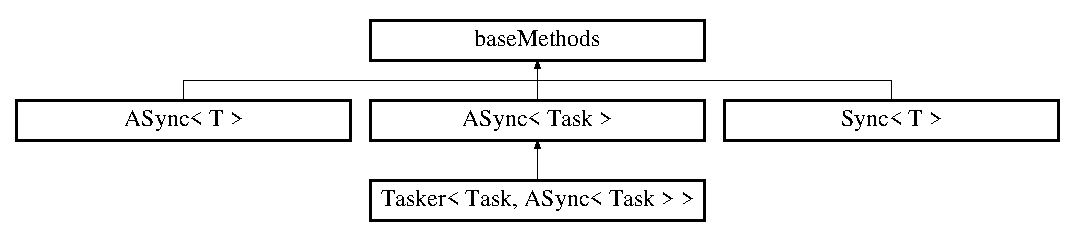
\includegraphics[height=2.731707cm]{classbase_methods}
\end{center}
\end{figure}
\subsection*{Public Member Functions}
\begin{DoxyCompactItemize}
\item 
\mbox{\Hypertarget{classbase_methods_a734354bd066339c46165903791f01e11}\label{classbase_methods_a734354bd066339c46165903791f01e11}} 
virtual void {\bfseries printprechar} (Stream \&stream)
\end{DoxyCompactItemize}


The documentation for this class was generated from the following file\+:\begin{DoxyCompactItemize}
\item 
src/\+Tasker/src/\hyperlink{_task_methods_8h}{Task\+Methods.\+h}\end{DoxyCompactItemize}

\hypertarget{class_e_s_pdevice_finder}{}\section{E\+S\+Pdevice\+Finder Class Reference}
\label{class_e_s_pdevice_finder}\index{E\+S\+Pdevice\+Finder@{E\+S\+Pdevice\+Finder}}
\subsection*{Classes}
\begin{DoxyCompactItemize}
\item 
struct \hyperlink{struct_e_s_pdevice_finder_1_1_u_d_p__item}{U\+D\+P\+\_\+item}
\end{DoxyCompactItemize}
\subsection*{Public Types}
\begin{DoxyCompactItemize}
\item 
\mbox{\Hypertarget{class_e_s_pdevice_finder_a200ecda9bb2d679f4b5d6f99fa76c7ab}\label{class_e_s_pdevice_finder_a200ecda9bb2d679f4b5d6f99fa76c7ab}} 
typedef std\+::list$<$ std\+::unique\+\_\+ptr$<$ \hyperlink{struct_e_s_pdevice_finder_1_1_u_d_p__item}{U\+D\+P\+\_\+item} $>$ $>$ {\bfseries U\+D\+P\+List}
\end{DoxyCompactItemize}
\subsection*{Public Member Functions}
\begin{DoxyCompactItemize}
\item 
\mbox{\Hypertarget{class_e_s_pdevice_finder_a539a9d277870c704fd16c3489734ea37}\label{class_e_s_pdevice_finder_a539a9d277870c704fd16c3489734ea37}} 
void {\bfseries begin} (const char $\ast$host=nullptr, uint16\+\_\+t port=0)
\item 
\mbox{\Hypertarget{class_e_s_pdevice_finder_adfd99b6f9fbb3f5f05eb7af1c73faa21}\label{class_e_s_pdevice_finder_adfd99b6f9fbb3f5f05eb7af1c73faa21}} 
void {\bfseries end} ()
\item 
\mbox{\Hypertarget{class_e_s_pdevice_finder_a562a409039e8e51c690669c7be3d44c6}\label{class_e_s_pdevice_finder_a562a409039e8e51c690669c7be3d44c6}} 
void {\bfseries set\+Host} (String host)
\item 
\mbox{\Hypertarget{class_e_s_pdevice_finder_a42ceb57b393c73104b2326d3b01be2ab}\label{class_e_s_pdevice_finder_a42ceb57b393c73104b2326d3b01be2ab}} 
void {\bfseries set\+App\+Name} (String app\+Name)
\item 
\mbox{\Hypertarget{class_e_s_pdevice_finder_ac3d5d4e47e6e74f4ebbf58edd1b5df86}\label{class_e_s_pdevice_finder_ac3d5d4e47e6e74f4ebbf58edd1b5df86}} 
void {\bfseries set\+Port} (uint16\+\_\+t port)
\item 
\mbox{\Hypertarget{class_e_s_pdevice_finder_abdb88ce6e272673b4ad53d2e60ef4d38}\label{class_e_s_pdevice_finder_abdb88ce6e272673b4ad53d2e60ef4d38}} 
void {\bfseries set\+Multicast\+IP} (I\+P\+Address addr)
\item 
\mbox{\Hypertarget{class_e_s_pdevice_finder_a24122d858746c2a78263643749744f63}\label{class_e_s_pdevice_finder_a24122d858746c2a78263643749744f63}} 
void {\bfseries filter\+By\+App\+Name} (bool value)
\item 
\mbox{\Hypertarget{class_e_s_pdevice_finder_a70330e8122313e4fd6758c157dde9eb9}\label{class_e_s_pdevice_finder_a70330e8122313e4fd6758c157dde9eb9}} 
void {\bfseries loop} ()
\item 
\mbox{\Hypertarget{class_e_s_pdevice_finder_a1d04d6073b194a78cffa11738bef8a1a}\label{class_e_s_pdevice_finder_a1d04d6073b194a78cffa11738bef8a1a}} 
void {\bfseries ping} ()
\item 
\mbox{\Hypertarget{class_e_s_pdevice_finder_a4a91d0e2f05a76d2d73a9ecc5bb53d3a}\label{class_e_s_pdevice_finder_a4a91d0e2f05a76d2d73a9ecc5bb53d3a}} 
uint8\+\_\+t {\bfseries count} ()
\item 
\mbox{\Hypertarget{class_e_s_pdevice_finder_a75fb47fe700aab08dc30740e093421e8}\label{class_e_s_pdevice_finder_a75fb47fe700aab08dc30740e093421e8}} 
const char $\ast$ {\bfseries get\+Name} (uint8\+\_\+t i)
\item 
\mbox{\Hypertarget{class_e_s_pdevice_finder_a169118a96c267f8ce73cecffdab2759b}\label{class_e_s_pdevice_finder_a169118a96c267f8ce73cecffdab2759b}} 
I\+P\+Address {\bfseries get\+IP} (uint8\+\_\+t i)
\item 
\mbox{\Hypertarget{class_e_s_pdevice_finder_a391e961c110cba87d250a0f151ee51a2}\label{class_e_s_pdevice_finder_a391e961c110cba87d250a0f151ee51a2}} 
void {\bfseries cache\+Results} (bool val)
\item 
\mbox{\Hypertarget{class_e_s_pdevice_finder_adbc71125eedd3791e9443b14cd1a320f}\label{class_e_s_pdevice_finder_adbc71125eedd3791e9443b14cd1a320f}} 
void {\bfseries clear\+Results} ()
\end{DoxyCompactItemize}


The documentation for this class was generated from the following files\+:\begin{DoxyCompactItemize}
\item 
src/\+E\+S\+Pdevice\+Finder/src/E\+S\+Pdevice\+Finder.\+h\item 
src/\+E\+S\+Pdevice\+Finder/src/E\+S\+Pdevice\+Finder.\+cpp\end{DoxyCompactItemize}

\hypertarget{class_e_s_pmanager}{}\section{E\+S\+Pmanager Class Reference}
\label{class_e_s_pmanager}\index{E\+S\+Pmanager@{E\+S\+Pmanager}}


{\ttfamily \#include $<$E\+S\+Pmanager.\+h$>$}

\subsection*{Public Member Functions}
\begin{DoxyCompactItemize}
\item 
\hyperlink{class_e_s_pmanager_ade34dcdb30c7577b56f46b03c38b83d8}{E\+S\+Pmanager} (Async\+Web\+Server \&H\+T\+TP, FS \&fs=S\+P\+I\+F\+FS)
\begin{DoxyCompactList}\small\item\em Constructor brief description. \end{DoxyCompactList}\item 
\mbox{\Hypertarget{class_e_s_pmanager_a3ffeee3a4596d0416b4294987e94cd54}\label{class_e_s_pmanager_a3ffeee3a4596d0416b4294987e94cd54}} 
E\+S\+P\+M\+A\+N\+\_\+\+E\+R\+R\+\_\+t {\bfseries begin} ()
\item 
\mbox{\Hypertarget{class_e_s_pmanager_a18e1632178c113906997626820767f1d}\label{class_e_s_pmanager_a18e1632178c113906997626820767f1d}} 
E\+S\+P\+M\+A\+N\+\_\+\+E\+R\+R\+\_\+t {\bfseries begin} (\hyperlink{class_e_s_p_m_a_n_1_1my_string}{my\+String} ssid, \hyperlink{class_e_s_p_m_a_n_1_1my_string}{my\+String} pass)
\item 
\mbox{\Hypertarget{class_e_s_pmanager_abc765bc38931480a69aa722703116568}\label{class_e_s_pmanager_abc765bc38931480a69aa722703116568}} 
void {\bfseries handle} ()
\item 
\mbox{\Hypertarget{class_e_s_pmanager_a2ac01b9cca5905187732d6c6eeee433c}\label{class_e_s_pmanager_a2ac01b9cca5905187732d6c6eeee433c}} 
String {\bfseries get\+Hostname} ()
\item 
\mbox{\Hypertarget{class_e_s_pmanager_a11531fbfd8fc09fad93435f8a99b5780}\label{class_e_s_pmanager_a11531fbfd8fc09fad93435f8a99b5780}} 
\hyperlink{class_e_s_p_m_a_n_1_1my_string}{my\+String} {\bfseries get\+Error} (E\+S\+P\+M\+A\+N\+\_\+\+E\+R\+R\+\_\+t err)
\item 
\mbox{\Hypertarget{class_e_s_pmanager_a7fe42a45697d67434a21e4fbf2201572}\label{class_e_s_pmanager_a7fe42a45697d67434a21e4fbf2201572}} 
\hyperlink{class_e_s_p_m_a_n_1_1my_string}{my\+String} {\bfseries get\+Error} (int err)
\item 
\mbox{\Hypertarget{class_e_s_pmanager_a8b05b608f891bbe67d3742d749620db8}\label{class_e_s_pmanager_a8b05b608f891bbe67d3742d749620db8}} 
uint32\+\_\+t {\bfseries true\+Sketch\+Size} ()
\item 
\mbox{\Hypertarget{class_e_s_pmanager_ac4cd153ca61c45180fa138431a2eaaf2}\label{class_e_s_pmanager_ac4cd153ca61c45180fa138431a2eaaf2}} 
String {\bfseries get\+Sketch\+M\+D5} ()
\item 
\mbox{\Hypertarget{class_e_s_pmanager_ad620b2481d8b8d575f21c8f70f069235}\label{class_e_s_pmanager_ad620b2481d8b8d575f21c8f70f069235}} 
Async\+Event\+Source \& {\bfseries get\+Event} ()
\item 
\mbox{\Hypertarget{class_e_s_pmanager_aaa81ea53d94f2ffce01ab0eb13902cc3}\label{class_e_s_pmanager_aaa81ea53d94f2ffce01ab0eb13902cc3}} 
bool {\bfseries event\+\_\+send} (\hyperlink{class_e_s_p_m_a_n_1_1my_string}{my\+String} topic, \hyperlink{class_e_s_p_m_a_n_1_1my_string}{my\+String} msg)
\item 
\mbox{\Hypertarget{class_e_s_pmanager_a0a5acca1b6d70a357774b07986c38ea5}\label{class_e_s_pmanager_a0a5acca1b6d70a357774b07986c38ea5}} 
E\+S\+P\+M\+A\+N\+\_\+\+E\+R\+R\+\_\+t {\bfseries upgrade} (String path=String(), bool runasync=true)
\item 
\mbox{\Hypertarget{class_e_s_pmanager_a5974ea776024c990c28376fd237515ed}\label{class_e_s_pmanager_a5974ea776024c990c28376fd237515ed}} 
void {\bfseries factory\+Reset} ()
\item 
\mbox{\Hypertarget{class_e_s_pmanager_ad1796ea349f45a0246f6d344f83f0614}\label{class_e_s_pmanager_ad1796ea349f45a0246f6d344f83f0614}} 
int {\bfseries save} ()
\item 
\mbox{\Hypertarget{class_e_s_pmanager_a9a8d0c15671c93f559ba6ab67c41a43f}\label{class_e_s_pmanager_a9a8d0c15671c93f559ba6ab67c41a43f}} 
bool {\bfseries portal} ()
\item 
\mbox{\Hypertarget{class_e_s_pmanager_a918d341439796101a03f7fd8105db9e6}\label{class_e_s_pmanager_a918d341439796101a03f7fd8105db9e6}} 
E\+S\+P\+M\+A\+N\+\_\+\+E\+R\+R\+\_\+t {\bfseries enable\+Portal} ()
\item 
\mbox{\Hypertarget{class_e_s_pmanager_a9c392a712f02fb7ca1c54783f7b45ab4}\label{class_e_s_pmanager_a9c392a712f02fb7ca1c54783f7b45ab4}} 
void {\bfseries disable\+Portal} ()
\item 
\mbox{\Hypertarget{class_e_s_pmanager_a8f715e70f0711cedafdd5b3f1b58aacb}\label{class_e_s_pmanager_a8f715e70f0711cedafdd5b3f1b58aacb}} 
\hyperlink{class_tasker}{A\+Sync\+Tasker} \& {\bfseries get\+Task\+Manager} ()
\item 
\mbox{\Hypertarget{class_e_s_pmanager_ab0858c128085f2bd12a17261e8fefe52}\label{class_e_s_pmanager_ab0858c128085f2bd12a17261e8fefe52}} 
\hyperlink{class_tasker}{A\+Sync\+Tasker} \& {\bfseries tasker} ()
\end{DoxyCompactItemize}
\subsection*{Static Public Member Functions}
\begin{DoxyCompactItemize}
\item 
\mbox{\Hypertarget{class_e_s_pmanager_acb4e20b06625138b15c0f39c3522d9ea}\label{class_e_s_pmanager_acb4e20b06625138b15c0f39c3522d9ea}} 
static String {\bfseries format\+Bytes} (size\+\_\+t bytes)
\item 
\mbox{\Hypertarget{class_e_s_pmanager_a73dc4833b3cd7bfbc6dfb81bee54ab36}\label{class_e_s_pmanager_a73dc4833b3cd7bfbc6dfb81bee54ab36}} 
static bool {\bfseries Stringto\+M\+AC} (uint8\+\_\+t $\ast$mac, const String \&input)
\item 
\mbox{\Hypertarget{class_e_s_pmanager_a354a5ab6a0c064c75809ce481bc0ba91}\label{class_e_s_pmanager_a354a5ab6a0c064c75809ce481bc0ba91}} 
static void {\bfseries urldecode} (char $\ast$dst, const char $\ast$src)
\item 
\mbox{\Hypertarget{class_e_s_pmanager_a6cfff38606f5ed12b49aada480b23cab}\label{class_e_s_pmanager_a6cfff38606f5ed12b49aada480b23cab}} 
static String {\bfseries file\+\_\+md5} (File \&f)
\item 
\mbox{\Hypertarget{class_e_s_pmanager_ade55619386f08492b0b6d4dbd2cf32c3}\label{class_e_s_pmanager_ade55619386f08492b0b6d4dbd2cf32c3}} 
{\footnotesize template$<$class T  = Json\+Object$>$ }\\static void {\bfseries send\+Jsonto\+H\+T\+TP} (const T \&root, Async\+Web\+Server\+Request $\ast$request)
\end{DoxyCompactItemize}


\subsection{Detailed Description}
\hyperlink{class_e_s_pmanager}{E\+S\+Pmanager} class -\/ Main instance 

\subsection{Constructor \& Destructor Documentation}
\mbox{\Hypertarget{class_e_s_pmanager_ade34dcdb30c7577b56f46b03c38b83d8}\label{class_e_s_pmanager_ade34dcdb30c7577b56f46b03c38b83d8}} 
\index{E\+S\+Pmanager@{E\+S\+Pmanager}!E\+S\+Pmanager@{E\+S\+Pmanager}}
\index{E\+S\+Pmanager@{E\+S\+Pmanager}!E\+S\+Pmanager@{E\+S\+Pmanager}}
\subsubsection{\texorpdfstring{E\+S\+Pmanager()}{ESPmanager()}}
{\footnotesize\ttfamily E\+S\+Pmanager\+::\+E\+S\+Pmanager (\begin{DoxyParamCaption}\item[{Async\+Web\+Server \&}]{H\+T\+TP,  }\item[{FS \&}]{fs = {\ttfamily SPIFFS} }\end{DoxyParamCaption})}



Constructor brief description. 

Pass in \href{https://github.com/me-no-dev/ESPAsyncWebServer}{\tt Async\+Web\+Server} and optionally the \href{http://esp8266.github.io/Arduino/versions/2.3.0-rc2/doc/filesystem.html#file-system-object-spiffs}{\tt S\+P\+I\+F\+FS} file system. By default it uses S\+P\+I\+F\+FS as per Arduino E\+S\+P8266 

The documentation for this class was generated from the following files\+:\begin{DoxyCompactItemize}
\item 
src/\hyperlink{_e_s_pmanager_8h}{E\+S\+Pmanager.\+h}\item 
src/\hyperlink{_e_s_pmanager_8cpp}{E\+S\+Pmanager.\+cpp}\end{DoxyCompactItemize}

\hypertarget{class_flash_writer}{}\section{Flash\+Writer Class Reference}
\label{class_flash_writer}\index{Flash\+Writer@{Flash\+Writer}}
Inheritance diagram for Flash\+Writer\+:\begin{figure}[H]
\begin{center}
\leavevmode
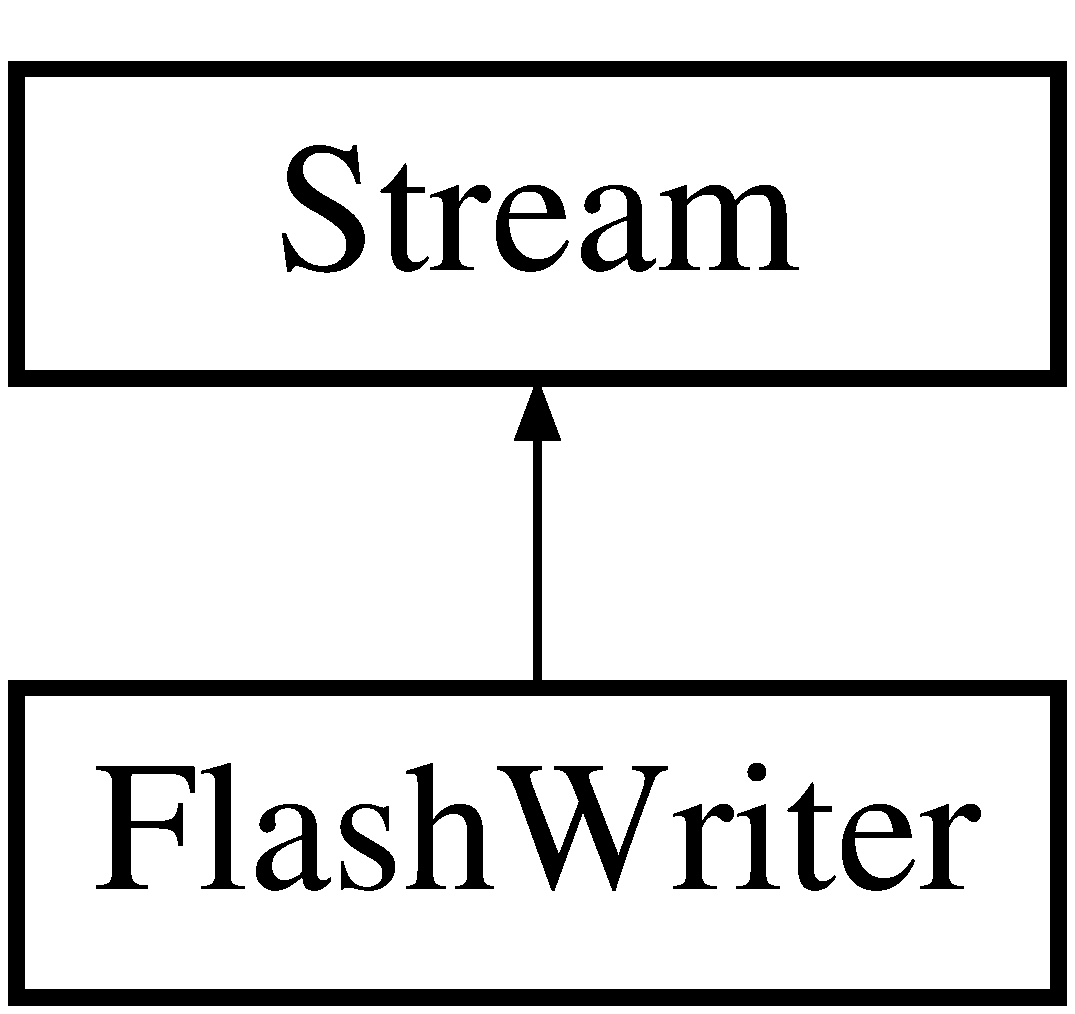
\includegraphics[height=2.000000cm]{class_flash_writer}
\end{center}
\end{figure}
\subsection*{Public Member Functions}
\begin{DoxyCompactItemize}
\item 
\mbox{\Hypertarget{class_flash_writer_a1376815be0390bdedfd3d59eda900732}\label{class_flash_writer_a1376815be0390bdedfd3d59eda900732}} 
bool {\bfseries begin} (size\+\_\+t size)
\item 
\mbox{\Hypertarget{class_flash_writer_a41447872c8c0ecb37bdd9bdae4fa8dc2}\label{class_flash_writer_a41447872c8c0ecb37bdd9bdae4fa8dc2}} 
bool {\bfseries is\+Running} ()
\item 
\mbox{\Hypertarget{class_flash_writer_a51781bc5e919454056cfaed0156873a3}\label{class_flash_writer_a51781bc5e919454056cfaed0156873a3}} 
bool {\bfseries is\+Finished} ()
\item 
\mbox{\Hypertarget{class_flash_writer_a18950100a30881380d55a348bd1e1526}\label{class_flash_writer_a18950100a30881380d55a348bd1e1526}} 
size\+\_\+t {\bfseries size} ()
\item 
\mbox{\Hypertarget{class_flash_writer_af395626466b39b7aed1da7598e1e2e67}\label{class_flash_writer_af395626466b39b7aed1da7598e1e2e67}} 
size\+\_\+t {\bfseries progress} ()
\item 
\mbox{\Hypertarget{class_flash_writer_a99c79273d8c09f12c9ad5a2c304fc346}\label{class_flash_writer_a99c79273d8c09f12c9ad5a2c304fc346}} 
size\+\_\+t {\bfseries remaining} ()
\item 
\mbox{\Hypertarget{class_flash_writer_a8a38cd9ac0b6fcd17e843d0b43e9f553}\label{class_flash_writer_a8a38cd9ac0b6fcd17e843d0b43e9f553}} 
String {\bfseries get\+M\+D5} ()
\item 
\mbox{\Hypertarget{class_flash_writer_a4dbb71d7dd54a7045f67cc7b9b67cfdb}\label{class_flash_writer_a4dbb71d7dd54a7045f67cc7b9b67cfdb}} 
void {\bfseries timeout} (uint32\+\_\+t value)
\item 
\mbox{\Hypertarget{class_flash_writer_aa22c6cb879da90b10d677fcd04fdf349}\label{class_flash_writer_aa22c6cb879da90b10d677fcd04fdf349}} 
virtual size\+\_\+t {\bfseries write} (const uint8\+\_\+t $\ast$data, size\+\_\+t len) override
\item 
\mbox{\Hypertarget{class_flash_writer_ad38210dcd95926ac5c9538a247580bff}\label{class_flash_writer_ad38210dcd95926ac5c9538a247580bff}} 
virtual size\+\_\+t {\bfseries write} (uint8\+\_\+t value) override
\item 
\mbox{\Hypertarget{class_flash_writer_ae77a296342ed2e6a182a47e3723ec793}\label{class_flash_writer_ae77a296342ed2e6a182a47e3723ec793}} 
virtual int {\bfseries available} () override
\item 
\mbox{\Hypertarget{class_flash_writer_a4663c0f6af43e917bdc3da3e713ce4d8}\label{class_flash_writer_a4663c0f6af43e917bdc3da3e713ce4d8}} 
virtual int {\bfseries read} () override
\item 
\mbox{\Hypertarget{class_flash_writer_aa28215079911b918877cf1bd48a19ca7}\label{class_flash_writer_aa28215079911b918877cf1bd48a19ca7}} 
virtual size\+\_\+t {\bfseries read\+Bytes} (uint8\+\_\+t $\ast$, size\+\_\+t)
\item 
\mbox{\Hypertarget{class_flash_writer_ab9a55816c9ae25b7a07c444ff93811d4}\label{class_flash_writer_ab9a55816c9ae25b7a07c444ff93811d4}} 
virtual int {\bfseries peek} () override
\item 
\mbox{\Hypertarget{class_flash_writer_a3d68a95de1159906ad910aa14530ff00}\label{class_flash_writer_a3d68a95de1159906ad910aa14530ff00}} 
virtual void {\bfseries flush} () override
\item 
\mbox{\Hypertarget{class_flash_writer_aeada2f4f7a906b30f0affce61551ad92}\label{class_flash_writer_aeada2f4f7a906b30f0affce61551ad92}} 
int {\bfseries write\+To\+Stream} (Stream $\ast$stream)
\end{DoxyCompactItemize}


The documentation for this class was generated from the following files\+:\begin{DoxyCompactItemize}
\item 
src/\hyperlink{_flash_writer_8h}{Flash\+Writer.\+h}\item 
src/\hyperlink{_flash_writer_8cpp}{Flash\+Writer.\+cpp}\end{DoxyCompactItemize}

\hypertarget{struct_e_s_p_m_a_n_1_1settings__t_1_1_g_e_n__t}{}\section{E\+S\+P\+M\+AN\+:\+:settings\+\_\+t\+:\+:G\+E\+N\+\_\+t Struct Reference}
\label{struct_e_s_p_m_a_n_1_1settings__t_1_1_g_e_n__t}\index{E\+S\+P\+M\+A\+N\+::settings\+\_\+t\+::\+G\+E\+N\+\_\+t@{E\+S\+P\+M\+A\+N\+::settings\+\_\+t\+::\+G\+E\+N\+\_\+t}}
\subsection*{Public Attributes}
\begin{DoxyCompactItemize}
\item 
\mbox{\Hypertarget{struct_e_s_p_m_a_n_1_1settings__t_1_1_g_e_n__t_aeec835601bc1c5f41299a036103091d8}\label{struct_e_s_p_m_a_n_1_1settings__t_1_1_g_e_n__t_aeec835601bc1c5f41299a036103091d8}} 
bool {\bfseries m\+D\+N\+Senabled} \{true\}
\item 
\mbox{\Hypertarget{struct_e_s_p_m_a_n_1_1settings__t_1_1_g_e_n__t_a8c99c150e6c95af13ef32ddd82d0627a}\label{struct_e_s_p_m_a_n_1_1settings__t_1_1_g_e_n__t_a8c99c150e6c95af13ef32ddd82d0627a}} 
\hyperlink{class_e_s_p_m_a_n_1_1my_string}{my\+String} {\bfseries host}
\item 
\mbox{\Hypertarget{struct_e_s_p_m_a_n_1_1settings__t_1_1_g_e_n__t_afaae059fdaaf04fe663a9349d0c50b8a}\label{struct_e_s_p_m_a_n_1_1settings__t_1_1_g_e_n__t_afaae059fdaaf04fe663a9349d0c50b8a}} 
\hyperlink{class_e_s_p_m_a_n_1_1my_string}{my\+String} {\bfseries update\+U\+RL}
\item 
\mbox{\Hypertarget{struct_e_s_p_m_a_n_1_1settings__t_1_1_g_e_n__t_a8324d39f9e52d23fd528629639d24ffe}\label{struct_e_s_p_m_a_n_1_1settings__t_1_1_g_e_n__t_a8324d39f9e52d23fd528629639d24ffe}} 
uint32\+\_\+t {\bfseries update\+Freq} \{0\}
\item 
\mbox{\Hypertarget{struct_e_s_p_m_a_n_1_1settings__t_1_1_g_e_n__t_a53523c29696b804a282f1da29eadcb48}\label{struct_e_s_p_m_a_n_1_1settings__t_1_1_g_e_n__t_a53523c29696b804a282f1da29eadcb48}} 
uint16\+\_\+t {\bfseries O\+T\+Aport} \{8266\}
\item 
\mbox{\Hypertarget{struct_e_s_p_m_a_n_1_1settings__t_1_1_g_e_n__t_a949188893480968881fb17c1b506d5c8}\label{struct_e_s_p_m_a_n_1_1settings__t_1_1_g_e_n__t_a949188893480968881fb17c1b506d5c8}} 
\hyperlink{class_e_s_p_m_a_n_1_1my_string}{my\+String} {\bfseries O\+T\+Apassword}
\item 
\mbox{\Hypertarget{struct_e_s_p_m_a_n_1_1settings__t_1_1_g_e_n__t_ae43e6322470d417489127577b03b3781}\label{struct_e_s_p_m_a_n_1_1settings__t_1_1_g_e_n__t_ae43e6322470d417489127577b03b3781}} 
\hyperlink{class_e_s_p_m_a_n_1_1my_string}{my\+String} {\bfseries G\+U\+Ihash}
\item 
\mbox{\Hypertarget{struct_e_s_p_m_a_n_1_1settings__t_1_1_g_e_n__t_a640bdf5adde684226a66dd298ac7efe5}\label{struct_e_s_p_m_a_n_1_1settings__t_1_1_g_e_n__t_a640bdf5adde684226a66dd298ac7efe5}} 
E\+S\+P\+M\+A\+N\+::ap\+\_\+boot\+\_\+mode\+\_\+t {\bfseries ap\+\_\+boot\+\_\+mode} \{E\+S\+P\+M\+A\+N\+::\+N\+O\+\_\+\+S\+T\+A\+\_\+\+B\+O\+OT\}
\item 
\mbox{\Hypertarget{struct_e_s_p_m_a_n_1_1settings__t_1_1_g_e_n__t_aa84d5a0388fc8068efa34d703deb329a}\label{struct_e_s_p_m_a_n_1_1settings__t_1_1_g_e_n__t_aa84d5a0388fc8068efa34d703deb329a}} 
E\+S\+P\+M\+A\+N\+::no\+\_\+sta\+\_\+mode\+\_\+t {\bfseries no\+\_\+sta\+\_\+mode} \{E\+S\+P\+M\+A\+N\+::\+N\+O\+\_\+\+S\+T\+A\+\_\+\+N\+O\+T\+H\+I\+NG\}
\item 
\mbox{\Hypertarget{struct_e_s_p_m_a_n_1_1settings__t_1_1_g_e_n__t_afc2c324995308d27e5ca2aad1e65d8e6}\label{struct_e_s_p_m_a_n_1_1settings__t_1_1_g_e_n__t_afc2c324995308d27e5ca2aad1e65d8e6}} 
bool {\bfseries O\+T\+Aupload} \{true\}
\item 
\mbox{\Hypertarget{struct_e_s_p_m_a_n_1_1settings__t_1_1_g_e_n__t_a48f40a1173569404329944f9ef57d951}\label{struct_e_s_p_m_a_n_1_1settings__t_1_1_g_e_n__t_a48f40a1173569404329944f9ef57d951}} 
bool {\bfseries portal} \{true\}
\item 
\mbox{\Hypertarget{struct_e_s_p_m_a_n_1_1settings__t_1_1_g_e_n__t_a352dd9cdbb9afecbf527047aa3786271}\label{struct_e_s_p_m_a_n_1_1settings__t_1_1_g_e_n__t_a352dd9cdbb9afecbf527047aa3786271}} 
bool {\bfseries usesyslog} \{false\}
\item 
\mbox{\Hypertarget{struct_e_s_p_m_a_n_1_1settings__t_1_1_g_e_n__t_a55b73ec450eda7d09e6a9afcd25e230f}\label{struct_e_s_p_m_a_n_1_1settings__t_1_1_g_e_n__t_a55b73ec450eda7d09e6a9afcd25e230f}} 
I\+P\+Address {\bfseries syslog\+IP}
\item 
\mbox{\Hypertarget{struct_e_s_p_m_a_n_1_1settings__t_1_1_g_e_n__t_ac0d72a4b8ed1054cb8a2325816cd82fa}\label{struct_e_s_p_m_a_n_1_1settings__t_1_1_g_e_n__t_ac0d72a4b8ed1054cb8a2325816cd82fa}} 
uint16\+\_\+t {\bfseries syslog\+Port} \{514\}
\item 
\mbox{\Hypertarget{struct_e_s_p_m_a_n_1_1settings__t_1_1_g_e_n__t_a17722c66b84759e24f2a3c0ae0bfe223}\label{struct_e_s_p_m_a_n_1_1settings__t_1_1_g_e_n__t_a17722c66b84759e24f2a3c0ae0bfe223}} 
uint8\+\_\+t {\bfseries syslog\+Proto} \{0\}
\end{DoxyCompactItemize}


The documentation for this struct was generated from the following file\+:\begin{DoxyCompactItemize}
\item 
src/\hyperlink{_e_s_p_m_a_n_8h}{E\+S\+P\+M\+A\+N.\+h}\end{DoxyCompactItemize}

\hypertarget{class_e_s_p_m_a_n_1_1_j_s_o_npackage}{}\section{E\+S\+P\+M\+AN\+:\+:J\+S\+O\+Npackage Class Reference}
\label{class_e_s_p_m_a_n_1_1_j_s_o_npackage}\index{E\+S\+P\+M\+A\+N\+::\+J\+S\+O\+Npackage@{E\+S\+P\+M\+A\+N\+::\+J\+S\+O\+Npackage}}
\subsection*{Public Member Functions}
\begin{DoxyCompactItemize}
\item 
\mbox{\Hypertarget{class_e_s_p_m_a_n_1_1_j_s_o_npackage_a2ccb4238cacc75894132f8d50f68e7ab}\label{class_e_s_p_m_a_n_1_1_j_s_o_npackage_a2ccb4238cacc75894132f8d50f68e7ab}} 
{\bfseries J\+S\+O\+Npackage} (bool is\+Array=false)
\item 
\mbox{\Hypertarget{class_e_s_p_m_a_n_1_1_j_s_o_npackage_aac25a41ff46bdbe8ffb7fa2734bf2b7e}\label{class_e_s_p_m_a_n_1_1_j_s_o_npackage_aac25a41ff46bdbe8ffb7fa2734bf2b7e}} 
Json\+Variant \& {\bfseries get\+Root} ()
\item 
\mbox{\Hypertarget{class_e_s_p_m_a_n_1_1_j_s_o_npackage_a108cba1a08b67062cb4673e9dc1b6cce}\label{class_e_s_p_m_a_n_1_1_j_s_o_npackage_a108cba1a08b67062cb4673e9dc1b6cce}} 
int {\bfseries parse\+S\+P\+I\+FS} (const char $\ast$file, FS \&fs=S\+P\+I\+F\+FS)
\item 
\mbox{\Hypertarget{class_e_s_p_m_a_n_1_1_j_s_o_npackage_a8bca1bff6ca00d696f8cbea49b06da4a}\label{class_e_s_p_m_a_n_1_1_j_s_o_npackage_a8bca1bff6ca00d696f8cbea49b06da4a}} 
int {\bfseries parse} (char $\ast$data, int size)
\item 
\mbox{\Hypertarget{class_e_s_p_m_a_n_1_1_j_s_o_npackage_a602fc85ee5b09b7d1eb7e08f3dbbe772}\label{class_e_s_p_m_a_n_1_1_j_s_o_npackage_a602fc85ee5b09b7d1eb7e08f3dbbe772}} 
bool {\bfseries save} (const char $\ast$file)
\end{DoxyCompactItemize}
\subsection*{Static Public Member Functions}
\begin{DoxyCompactItemize}
\item 
\mbox{\Hypertarget{class_e_s_p_m_a_n_1_1_j_s_o_npackage_a6eb74788124b334b2c9da777867f1ca2}\label{class_e_s_p_m_a_n_1_1_j_s_o_npackage_a6eb74788124b334b2c9da777867f1ca2}} 
static void {\bfseries mergejson} (Json\+Object \&dest, Json\+Object \&src)
\end{DoxyCompactItemize}


The documentation for this class was generated from the following files\+:\begin{DoxyCompactItemize}
\item 
src/\hyperlink{_e_s_p_m_a_n_8h}{E\+S\+P\+M\+A\+N.\+h}\item 
src/\hyperlink{_e_s_p_m_a_n_8cpp}{E\+S\+P\+M\+A\+N.\+cpp}\end{DoxyCompactItemize}

\hypertarget{class_e_s_p_m_a_n_1_1my_string}{}\section{E\+S\+P\+M\+AN\+:\+:my\+String Class Reference}
\label{class_e_s_p_m_a_n_1_1my_string}\index{E\+S\+P\+M\+A\+N\+::my\+String@{E\+S\+P\+M\+A\+N\+::my\+String}}
Inheritance diagram for E\+S\+P\+M\+AN\+:\+:my\+String\+:\begin{figure}[H]
\begin{center}
\leavevmode
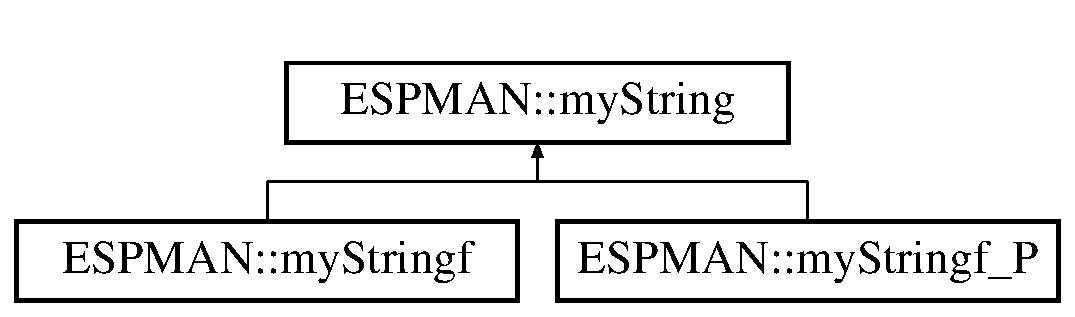
\includegraphics[height=2.000000cm]{class_e_s_p_m_a_n_1_1my_string}
\end{center}
\end{figure}
\subsection*{Public Member Functions}
\begin{DoxyCompactItemize}
\item 
\mbox{\Hypertarget{class_e_s_p_m_a_n_1_1my_string_afc1775fa29859a087342ca597683d147}\label{class_e_s_p_m_a_n_1_1my_string_afc1775fa29859a087342ca597683d147}} 
{\bfseries my\+String} (const char $\ast$cstr)
\item 
\mbox{\Hypertarget{class_e_s_p_m_a_n_1_1my_string_adcc74eb7f9d25ba712f1e8bd5229d942}\label{class_e_s_p_m_a_n_1_1my_string_adcc74eb7f9d25ba712f1e8bd5229d942}} 
{\bfseries my\+String} (const \hyperlink{class_e_s_p_m_a_n_1_1my_string}{my\+String} \&str)
\item 
\mbox{\Hypertarget{class_e_s_p_m_a_n_1_1my_string_a2819cbc1107839752bcf6c27afa25bb4}\label{class_e_s_p_m_a_n_1_1my_string_a2819cbc1107839752bcf6c27afa25bb4}} 
{\bfseries my\+String} (\hyperlink{class_e_s_p_m_a_n_1_1my_string}{my\+String} \&\&str)
\item 
\mbox{\Hypertarget{class_e_s_p_m_a_n_1_1my_string_abd5065ad2d08a4ec16cec6a06fbb4e61}\label{class_e_s_p_m_a_n_1_1my_string_abd5065ad2d08a4ec16cec6a06fbb4e61}} 
{\bfseries my\+String} (const \+\_\+\+\_\+\+Flash\+String\+Helper $\ast$str)
\item 
\mbox{\Hypertarget{class_e_s_p_m_a_n_1_1my_string_a36e9284352bf1a9237887aa6d7d28492}\label{class_e_s_p_m_a_n_1_1my_string_a36e9284352bf1a9237887aa6d7d28492}} 
{\bfseries my\+String} (String str)
\item 
\mbox{\Hypertarget{class_e_s_p_m_a_n_1_1my_string_a56252d20748d05a52157b1aa485a144f}\label{class_e_s_p_m_a_n_1_1my_string_a56252d20748d05a52157b1aa485a144f}} 
{\bfseries my\+String} (nullptr\+\_\+t ptr)
\item 
\mbox{\Hypertarget{class_e_s_p_m_a_n_1_1my_string_a6f326c837975dac31d99934c21345dab}\label{class_e_s_p_m_a_n_1_1my_string_a6f326c837975dac31d99934c21345dab}} 
\hyperlink{class_e_s_p_m_a_n_1_1my_string}{my\+String} \& {\bfseries operator=} (const char $\ast$cstr)
\item 
\mbox{\Hypertarget{class_e_s_p_m_a_n_1_1my_string_ab763c8547a0476325cb638290073c070}\label{class_e_s_p_m_a_n_1_1my_string_ab763c8547a0476325cb638290073c070}} 
\hyperlink{class_e_s_p_m_a_n_1_1my_string}{my\+String} \& {\bfseries operator=} (const \+\_\+\+\_\+\+Flash\+String\+Helper $\ast$str)
\item 
\mbox{\Hypertarget{class_e_s_p_m_a_n_1_1my_string_abeb7f40366b22e04ffb133726247989c}\label{class_e_s_p_m_a_n_1_1my_string_abeb7f40366b22e04ffb133726247989c}} 
\hyperlink{class_e_s_p_m_a_n_1_1my_string}{my\+String} \& {\bfseries operator=} (const \hyperlink{class_e_s_p_m_a_n_1_1my_string}{my\+String} \&str)
\item 
\mbox{\Hypertarget{class_e_s_p_m_a_n_1_1my_string_a7e420109dcb5a6eab4ff204d93108431}\label{class_e_s_p_m_a_n_1_1my_string_a7e420109dcb5a6eab4ff204d93108431}} 
\hyperlink{class_e_s_p_m_a_n_1_1my_string}{my\+String} \& {\bfseries operator=} (\hyperlink{class_e_s_p_m_a_n_1_1my_string}{my\+String} \&\&str)
\item 
\mbox{\Hypertarget{class_e_s_p_m_a_n_1_1my_string_a10b9e8d3a8265bc3dba062dd79fd824e}\label{class_e_s_p_m_a_n_1_1my_string_a10b9e8d3a8265bc3dba062dd79fd824e}} 
bool {\bfseries operator==} (const \hyperlink{class_e_s_p_m_a_n_1_1my_string}{my\+String} \&rhs)
\item 
\mbox{\Hypertarget{class_e_s_p_m_a_n_1_1my_string_ac578ab49440b8e207d6aff1b13814f5f}\label{class_e_s_p_m_a_n_1_1my_string_ac578ab49440b8e207d6aff1b13814f5f}} 
bool {\bfseries operator!=} (const \hyperlink{class_e_s_p_m_a_n_1_1my_string}{my\+String} \&rhs)
\item 
\mbox{\Hypertarget{class_e_s_p_m_a_n_1_1my_string_a8f21c84e1613a248203b2179fa9ab75f}\label{class_e_s_p_m_a_n_1_1my_string_a8f21c84e1613a248203b2179fa9ab75f}} 
const char $\ast$ {\bfseries operator()} () const
\item 
\mbox{\Hypertarget{class_e_s_p_m_a_n_1_1my_string_aaf8e0b8509fd6d1201d3d27f2ec23ab3}\label{class_e_s_p_m_a_n_1_1my_string_aaf8e0b8509fd6d1201d3d27f2ec23ab3}} 
const char $\ast$ {\bfseries operator()} (const char $\ast$) const
\item 
\mbox{\Hypertarget{class_e_s_p_m_a_n_1_1my_string_a1c423d16e99ff41c9a230258710c6510}\label{class_e_s_p_m_a_n_1_1my_string_a1c423d16e99ff41c9a230258710c6510}} 
const char $\ast$ {\bfseries c\+\_\+str} () const
\item 
\mbox{\Hypertarget{class_e_s_p_m_a_n_1_1my_string_a80ea963f812af38a1150dca96f9c2b23}\label{class_e_s_p_m_a_n_1_1my_string_a80ea963f812af38a1150dca96f9c2b23}} 
{\bfseries operator bool} () const
\item 
\mbox{\Hypertarget{class_e_s_p_m_a_n_1_1my_string_a7ef5f739cb0157ac3f9d5128ef722d63}\label{class_e_s_p_m_a_n_1_1my_string_a7ef5f739cb0157ac3f9d5128ef722d63}} 
{\bfseries operator String} () const
\end{DoxyCompactItemize}
\subsection*{Static Public Attributes}
\begin{DoxyCompactItemize}
\item 
\mbox{\Hypertarget{class_e_s_p_m_a_n_1_1my_string_adfdf69c1c7138db02cb425c546c61716}\label{class_e_s_p_m_a_n_1_1my_string_adfdf69c1c7138db02cb425c546c61716}} 
static const char $\ast$ {\bfseries \+\_\+null\+String} = \char`\"{}null\char`\"{}
\end{DoxyCompactItemize}
\subsection*{Protected Attributes}
\begin{DoxyCompactItemize}
\item 
\mbox{\Hypertarget{class_e_s_p_m_a_n_1_1my_string_af25573b872653fe4b868a41b21336466}\label{class_e_s_p_m_a_n_1_1my_string_af25573b872653fe4b868a41b21336466}} 
char $\ast$ {\bfseries buffer} \{nullptr\}
\end{DoxyCompactItemize}


The documentation for this class was generated from the following files\+:\begin{DoxyCompactItemize}
\item 
src/\hyperlink{_e_s_p_m_a_n_8h}{E\+S\+P\+M\+A\+N.\+h}\item 
src/\hyperlink{_e_s_p_m_a_n_8cpp}{E\+S\+P\+M\+A\+N.\+cpp}\end{DoxyCompactItemize}

\hypertarget{class_e_s_p_m_a_n_1_1my_stringf}{}\section{E\+S\+P\+M\+AN\+:\+:my\+Stringf Class Reference}
\label{class_e_s_p_m_a_n_1_1my_stringf}\index{E\+S\+P\+M\+A\+N\+::my\+Stringf@{E\+S\+P\+M\+A\+N\+::my\+Stringf}}
Inheritance diagram for E\+S\+P\+M\+AN\+:\+:my\+Stringf\+:\begin{figure}[H]
\begin{center}
\leavevmode
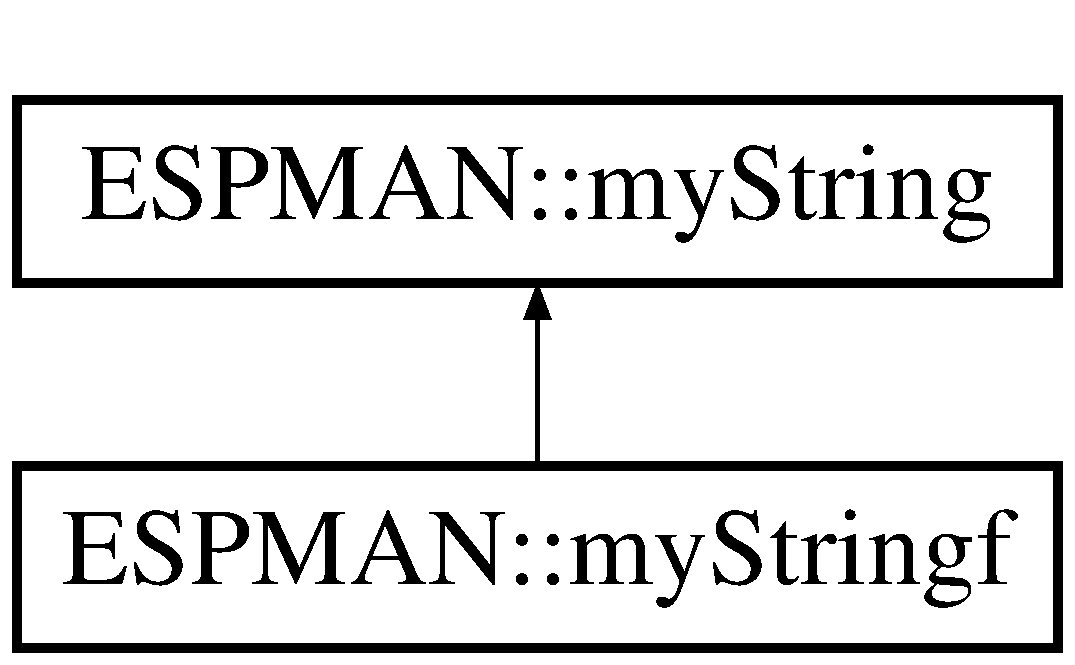
\includegraphics[height=2.000000cm]{class_e_s_p_m_a_n_1_1my_stringf}
\end{center}
\end{figure}
\subsection*{Public Member Functions}
\begin{DoxyCompactItemize}
\item 
\mbox{\Hypertarget{class_e_s_p_m_a_n_1_1my_stringf_a813bf9ec5007da9c6b4ad1026a8e2983}\label{class_e_s_p_m_a_n_1_1my_stringf_a813bf9ec5007da9c6b4ad1026a8e2983}} 
{\bfseries my\+Stringf} (const char $\ast$,...)
\item 
\mbox{\Hypertarget{class_e_s_p_m_a_n_1_1my_stringf_a5ca16b84f917e7bf72058aa929540611}\label{class_e_s_p_m_a_n_1_1my_stringf_a5ca16b84f917e7bf72058aa929540611}} 
{\bfseries my\+Stringf} (const \+\_\+\+\_\+\+Flash\+String\+Helper $\ast$,...)
\end{DoxyCompactItemize}
\subsection*{Additional Inherited Members}


The documentation for this class was generated from the following files\+:\begin{DoxyCompactItemize}
\item 
src/\hyperlink{_e_s_p_m_a_n_8h}{E\+S\+P\+M\+A\+N.\+h}\item 
src/\hyperlink{_e_s_p_m_a_n_8cpp}{E\+S\+P\+M\+A\+N.\+cpp}\end{DoxyCompactItemize}

\hypertarget{class_e_s_p_m_a_n_1_1my_stringf___p}{}\section{E\+S\+P\+M\+AN\+:\+:my\+Stringf\+\_\+P Class Reference}
\label{class_e_s_p_m_a_n_1_1my_stringf___p}\index{E\+S\+P\+M\+A\+N\+::my\+Stringf\+\_\+P@{E\+S\+P\+M\+A\+N\+::my\+Stringf\+\_\+P}}
Inheritance diagram for E\+S\+P\+M\+AN\+:\+:my\+Stringf\+\_\+P\+:\begin{figure}[H]
\begin{center}
\leavevmode
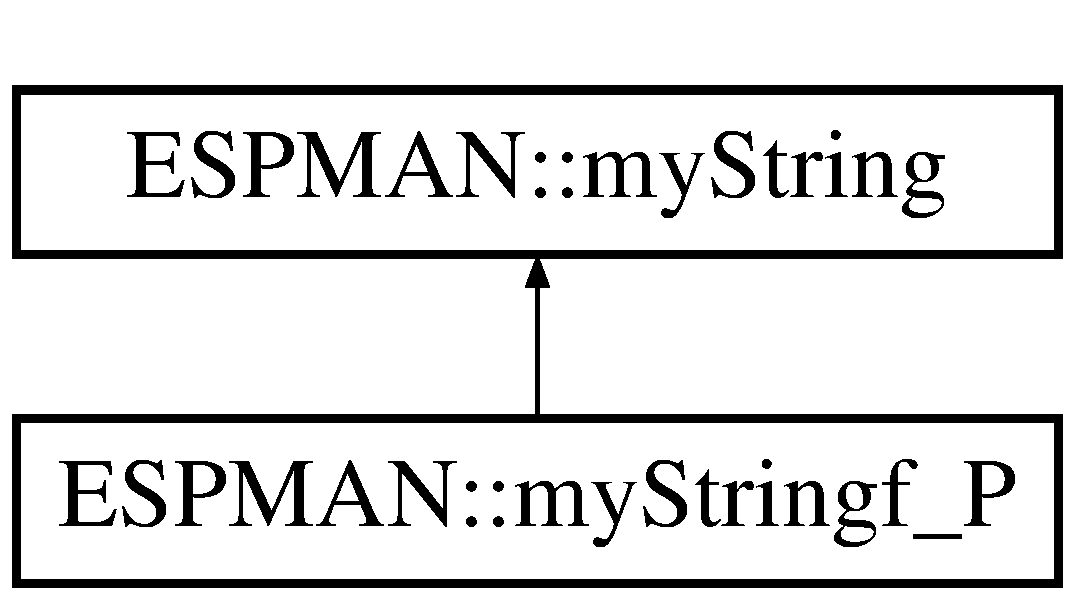
\includegraphics[height=2.000000cm]{class_e_s_p_m_a_n_1_1my_stringf___p}
\end{center}
\end{figure}
\subsection*{Public Member Functions}
\begin{DoxyCompactItemize}
\item 
\mbox{\Hypertarget{class_e_s_p_m_a_n_1_1my_stringf___p_acbb36a46a80ac34817f50747970912c1}\label{class_e_s_p_m_a_n_1_1my_stringf___p_acbb36a46a80ac34817f50747970912c1}} 
{\bfseries my\+Stringf\+\_\+P} (P\+G\+M\+\_\+P,...)
\end{DoxyCompactItemize}
\subsection*{Additional Inherited Members}


The documentation for this class was generated from the following files\+:\begin{DoxyCompactItemize}
\item 
src/\hyperlink{_e_s_p_m_a_n_8h}{E\+S\+P\+M\+A\+N.\+h}\item 
src/\hyperlink{_e_s_p_m_a_n_8cpp}{E\+S\+P\+M\+A\+N.\+cpp}\end{DoxyCompactItemize}

\hypertarget{struct_e_s_p_m_a_n_1_1password__t}{}\section{E\+S\+P\+M\+AN\+:\+:password\+\_\+t Struct Reference}
\label{struct_e_s_p_m_a_n_1_1password__t}\index{E\+S\+P\+M\+A\+N\+::password\+\_\+t@{E\+S\+P\+M\+A\+N\+::password\+\_\+t}}
\subsection*{Public Attributes}
\begin{DoxyCompactItemize}
\item 
\mbox{\Hypertarget{struct_e_s_p_m_a_n_1_1password__t_aa72bffbde591a99bf33ffdcd5cf14d28}\label{struct_e_s_p_m_a_n_1_1password__t_aa72bffbde591a99bf33ffdcd5cf14d28}} 
\hyperlink{class_e_s_p_m_a_n_1_1my_string}{my\+String} {\bfseries pass}
\item 
\mbox{\Hypertarget{struct_e_s_p_m_a_n_1_1password__t_a313d3a4c2f6fb251d5e2041211150d75}\label{struct_e_s_p_m_a_n_1_1password__t_a313d3a4c2f6fb251d5e2041211150d75}} 
\hyperlink{class_e_s_p_m_a_n_1_1my_string}{my\+String} {\bfseries salt}
\item 
\mbox{\Hypertarget{struct_e_s_p_m_a_n_1_1password__t_a08bdd3806d53dadfd6f4e672b73892c9}\label{struct_e_s_p_m_a_n_1_1password__t_a08bdd3806d53dadfd6f4e672b73892c9}} 
\hyperlink{class_e_s_p_m_a_n_1_1my_string}{my\+String} {\bfseries hash}
\end{DoxyCompactItemize}


The documentation for this struct was generated from the following file\+:\begin{DoxyCompactItemize}
\item 
src/\hyperlink{_e_s_p_m_a_n_8h}{E\+S\+P\+M\+A\+N.\+h}\end{DoxyCompactItemize}

\hypertarget{struct_e_s_p_m_a_n_1_1settings__t}{}\section{E\+S\+P\+M\+AN\+:\+:settings\+\_\+t Struct Reference}
\label{struct_e_s_p_m_a_n_1_1settings__t}\index{E\+S\+P\+M\+A\+N\+::settings\+\_\+t@{E\+S\+P\+M\+A\+N\+::settings\+\_\+t}}
\subsection*{Classes}
\begin{DoxyCompactItemize}
\item 
struct \hyperlink{struct_e_s_p_m_a_n_1_1settings__t_1_1_a_p__t}{A\+P\+\_\+t}
\item 
struct \hyperlink{struct_e_s_p_m_a_n_1_1settings__t_1_1_g_e_n__t}{G\+E\+N\+\_\+t}
\item 
struct \hyperlink{struct_e_s_p_m_a_n_1_1settings__t_1_1_s_t_a__t}{S\+T\+A\+\_\+t}
\end{DoxyCompactItemize}
\subsection*{Public Attributes}
\begin{DoxyCompactItemize}
\item 
\mbox{\Hypertarget{struct_e_s_p_m_a_n_1_1settings__t_afdfbe5e2138f651b5331ba75280dbc0d}\label{struct_e_s_p_m_a_n_1_1settings__t_afdfbe5e2138f651b5331ba75280dbc0d}} 
uint32\+\_\+t {\bfseries start\+\_\+time} \{0\}
\item 
\mbox{\Hypertarget{struct_e_s_p_m_a_n_1_1settings__t_a62838fac4146714011ede8f41437dec3}\label{struct_e_s_p_m_a_n_1_1settings__t_a62838fac4146714011ede8f41437dec3}} 
bool {\bfseries configured} \{false\}
\item 
\mbox{\Hypertarget{struct_e_s_p_m_a_n_1_1settings__t_ae4f94725baa4ef750e25da497c5a1e1e}\label{struct_e_s_p_m_a_n_1_1settings__t_ae4f94725baa4ef750e25da497c5a1e1e}} 
bool {\bfseries changed} \{false\}
\item 
\mbox{\Hypertarget{struct_e_s_p_m_a_n_1_1settings__t_aa89be6706c844d02a89be015f544f439}\label{struct_e_s_p_m_a_n_1_1settings__t_aa89be6706c844d02a89be015f544f439}} 
struct \hyperlink{struct_e_s_p_m_a_n_1_1settings__t_1_1_a_p__t}{E\+S\+P\+M\+A\+N\+::settings\+\_\+t\+::\+A\+P\+\_\+t} {\bfseries AP}
\item 
\mbox{\Hypertarget{struct_e_s_p_m_a_n_1_1settings__t_aa612b5cad39f6d7978e25de947dc9b8e}\label{struct_e_s_p_m_a_n_1_1settings__t_aa612b5cad39f6d7978e25de947dc9b8e}} 
struct \hyperlink{struct_e_s_p_m_a_n_1_1settings__t_1_1_s_t_a__t}{E\+S\+P\+M\+A\+N\+::settings\+\_\+t\+::\+S\+T\+A\+\_\+t} {\bfseries S\+TA}
\item 
\mbox{\Hypertarget{struct_e_s_p_m_a_n_1_1settings__t_abf8d25d5369c83792a31bc4e8b8ca9d5}\label{struct_e_s_p_m_a_n_1_1settings__t_abf8d25d5369c83792a31bc4e8b8ca9d5}} 
struct \hyperlink{struct_e_s_p_m_a_n_1_1settings__t_1_1_g_e_n__t}{E\+S\+P\+M\+A\+N\+::settings\+\_\+t\+::\+G\+E\+N\+\_\+t} {\bfseries G\+EN}
\end{DoxyCompactItemize}


The documentation for this struct was generated from the following file\+:\begin{DoxyCompactItemize}
\item 
src/\hyperlink{_e_s_p_m_a_n_8h}{E\+S\+P\+M\+A\+N.\+h}\end{DoxyCompactItemize}

\hypertarget{class_simple_task}{}\section{Simple\+Task Class Reference}
\label{class_simple_task}\index{Simple\+Task@{Simple\+Task}}
\subsection*{Public Types}
\begin{DoxyCompactItemize}
\item 
\mbox{\Hypertarget{class_simple_task_a26b575f2615e0e7e9214f8924d2afa16}\label{class_simple_task_a26b575f2615e0e7e9214f8924d2afa16}} 
typedef std\+::function$<$ void(\hyperlink{class_simple_task}{Simple\+Task} \&)$>$ {\bfseries tasker\+Cb\+\_\+t}
\end{DoxyCompactItemize}
\subsection*{Public Member Functions}
\begin{DoxyCompactItemize}
\item 
\mbox{\Hypertarget{class_simple_task_a64e20a96ac8a8a1e76de199890974818}\label{class_simple_task_a64e20a96ac8a8a1e76de199890974818}} 
{\bfseries Simple\+Task} (tasker\+Cb\+\_\+t cb, bool use\+Micros=false)
\item 
\mbox{\Hypertarget{class_simple_task_ac33dade916a8fc5c7050e1bdd793a396}\label{class_simple_task_ac33dade916a8fc5c7050e1bdd793a396}} 
bool {\bfseries run} (const uint8\+\_\+t priority=0)
\item 
\mbox{\Hypertarget{class_simple_task_a89a52e8151b087c1feb733a5799e76cb}\label{class_simple_task_a89a52e8151b087c1feb733a5799e76cb}} 
\hyperlink{class_simple_task}{Simple\+Task} \& {\bfseries set\+Timeout} (uint32\+\_\+t timeout)
\item 
\mbox{\Hypertarget{class_simple_task_ad86b716df71dd331df49294932a35a66}\label{class_simple_task_ad86b716df71dd331df49294932a35a66}} 
\hyperlink{class_simple_task}{Simple\+Task} \& {\bfseries set\+Repeat} (bool repeat=true)
\item 
\mbox{\Hypertarget{class_simple_task_acc38025a5a829da2c9df2720bb512c38}\label{class_simple_task_acc38025a5a829da2c9df2720bb512c38}} 
\hyperlink{class_simple_task}{Simple\+Task} \& {\bfseries enable} (bool val=true)
\item 
\mbox{\Hypertarget{class_simple_task_a7578873e52df9667d22523ea7fecab7e}\label{class_simple_task_a7578873e52df9667d22523ea7fecab7e}} 
\hyperlink{class_simple_task}{Simple\+Task} \& {\bfseries reset} ()
\end{DoxyCompactItemize}


The documentation for this class was generated from the following file\+:\begin{DoxyCompactItemize}
\item 
src/\+Tasker/src/\hyperlink{_task_8h}{Task.\+h}\end{DoxyCompactItemize}

\hypertarget{struct_e_s_p_m_a_n_1_1settings__t_1_1_s_t_a__t}{}\section{E\+S\+P\+M\+AN\+:\+:settings\+\_\+t\+:\+:S\+T\+A\+\_\+t Struct Reference}
\label{struct_e_s_p_m_a_n_1_1settings__t_1_1_s_t_a__t}\index{E\+S\+P\+M\+A\+N\+::settings\+\_\+t\+::\+S\+T\+A\+\_\+t@{E\+S\+P\+M\+A\+N\+::settings\+\_\+t\+::\+S\+T\+A\+\_\+t}}
\subsection*{Public Attributes}
\begin{DoxyCompactItemize}
\item 
\mbox{\Hypertarget{struct_e_s_p_m_a_n_1_1settings__t_1_1_s_t_a__t_a1629e9098ea8018d23e595d8050cd871}\label{struct_e_s_p_m_a_n_1_1settings__t_1_1_s_t_a__t_a1629e9098ea8018d23e595d8050cd871}} 
bool {\bfseries enabled} \{false\}
\item 
\mbox{\Hypertarget{struct_e_s_p_m_a_n_1_1settings__t_1_1_s_t_a__t_ab13e8466f7804c224fc14425eae0165a}\label{struct_e_s_p_m_a_n_1_1settings__t_1_1_s_t_a__t_ab13e8466f7804c224fc14425eae0165a}} 
bool {\bfseries has\+Config} \{false\}
\item 
\mbox{\Hypertarget{struct_e_s_p_m_a_n_1_1settings__t_1_1_s_t_a__t_ac5ca80bc6a2907b517c5303dedb86009}\label{struct_e_s_p_m_a_n_1_1settings__t_1_1_s_t_a__t_ac5ca80bc6a2907b517c5303dedb86009}} 
bool {\bfseries has\+M\+AC} \{false\}
\item 
\mbox{\Hypertarget{struct_e_s_p_m_a_n_1_1settings__t_1_1_s_t_a__t_a80a48aa98000550645554c119a8dd1b5}\label{struct_e_s_p_m_a_n_1_1settings__t_1_1_s_t_a__t_a80a48aa98000550645554c119a8dd1b5}} 
bool {\bfseries dhcp} \{true\}
\item 
\mbox{\Hypertarget{struct_e_s_p_m_a_n_1_1settings__t_1_1_s_t_a__t_a1c4226b0b842943ca037273746a552ce}\label{struct_e_s_p_m_a_n_1_1settings__t_1_1_s_t_a__t_a1c4226b0b842943ca037273746a552ce}} 
\hyperlink{class_e_s_p_m_a_n_1_1my_string}{my\+String} {\bfseries ssid}
\item 
\mbox{\Hypertarget{struct_e_s_p_m_a_n_1_1settings__t_1_1_s_t_a__t_a338bfbdb39021a7f4b008a60dd2b763e}\label{struct_e_s_p_m_a_n_1_1settings__t_1_1_s_t_a__t_a338bfbdb39021a7f4b008a60dd2b763e}} 
\hyperlink{class_e_s_p_m_a_n_1_1my_string}{my\+String} {\bfseries pass}
\item 
\mbox{\Hypertarget{struct_e_s_p_m_a_n_1_1settings__t_1_1_s_t_a__t_a7a8072be2bf18b6330ab6431b62673b1}\label{struct_e_s_p_m_a_n_1_1settings__t_1_1_s_t_a__t_a7a8072be2bf18b6330ab6431b62673b1}} 
I\+P\+Address {\bfseries IP}
\item 
\mbox{\Hypertarget{struct_e_s_p_m_a_n_1_1settings__t_1_1_s_t_a__t_a47d32faabfad4f78e936d66ada8f87a6}\label{struct_e_s_p_m_a_n_1_1settings__t_1_1_s_t_a__t_a47d32faabfad4f78e936d66ada8f87a6}} 
I\+P\+Address {\bfseries GW}
\item 
\mbox{\Hypertarget{struct_e_s_p_m_a_n_1_1settings__t_1_1_s_t_a__t_a1f5941fa03fd982bb3c6b6e3e49d422d}\label{struct_e_s_p_m_a_n_1_1settings__t_1_1_s_t_a__t_a1f5941fa03fd982bb3c6b6e3e49d422d}} 
I\+P\+Address {\bfseries SN}
\item 
\mbox{\Hypertarget{struct_e_s_p_m_a_n_1_1settings__t_1_1_s_t_a__t_a47c05877fc45751b9e2862ff1e604339}\label{struct_e_s_p_m_a_n_1_1settings__t_1_1_s_t_a__t_a47c05877fc45751b9e2862ff1e604339}} 
I\+P\+Address {\bfseries D\+N\+S1}
\item 
\mbox{\Hypertarget{struct_e_s_p_m_a_n_1_1settings__t_1_1_s_t_a__t_a777b5f40f4cd81c6eb34f95f1371e559}\label{struct_e_s_p_m_a_n_1_1settings__t_1_1_s_t_a__t_a777b5f40f4cd81c6eb34f95f1371e559}} 
I\+P\+Address {\bfseries D\+N\+S2}
\item 
\mbox{\Hypertarget{struct_e_s_p_m_a_n_1_1settings__t_1_1_s_t_a__t_a05c5a7392a52acdb595d1dfb1513ff7e}\label{struct_e_s_p_m_a_n_1_1settings__t_1_1_s_t_a__t_a05c5a7392a52acdb595d1dfb1513ff7e}} 
uint8\+\_\+t {\bfseries M\+AC} \mbox{[}6\mbox{]} = \{\textquotesingle{}\textbackslash{}0\textquotesingle{}\}
\item 
\mbox{\Hypertarget{struct_e_s_p_m_a_n_1_1settings__t_1_1_s_t_a__t_aef7cd00725794bf8466c26b0904fabe8}\label{struct_e_s_p_m_a_n_1_1settings__t_1_1_s_t_a__t_aef7cd00725794bf8466c26b0904fabe8}} 
bool {\bfseries auto\+Connect} \{true\}
\item 
\mbox{\Hypertarget{struct_e_s_p_m_a_n_1_1settings__t_1_1_s_t_a__t_a1b888df40cfad8366bb19723a5808f55}\label{struct_e_s_p_m_a_n_1_1settings__t_1_1_s_t_a__t_a1b888df40cfad8366bb19723a5808f55}} 
bool {\bfseries auto\+Reconnect} \{true\}
\end{DoxyCompactItemize}


The documentation for this struct was generated from the following file\+:\begin{DoxyCompactItemize}
\item 
src/\hyperlink{_e_s_p_m_a_n_8h}{E\+S\+P\+M\+A\+N.\+h}\end{DoxyCompactItemize}

\hypertarget{class_sync}{}\section{Sync$<$ T $>$ Class Template Reference}
\label{class_sync}\index{Sync$<$ T $>$@{Sync$<$ T $>$}}
Inheritance diagram for Sync$<$ T $>$\+:\begin{figure}[H]
\begin{center}
\leavevmode
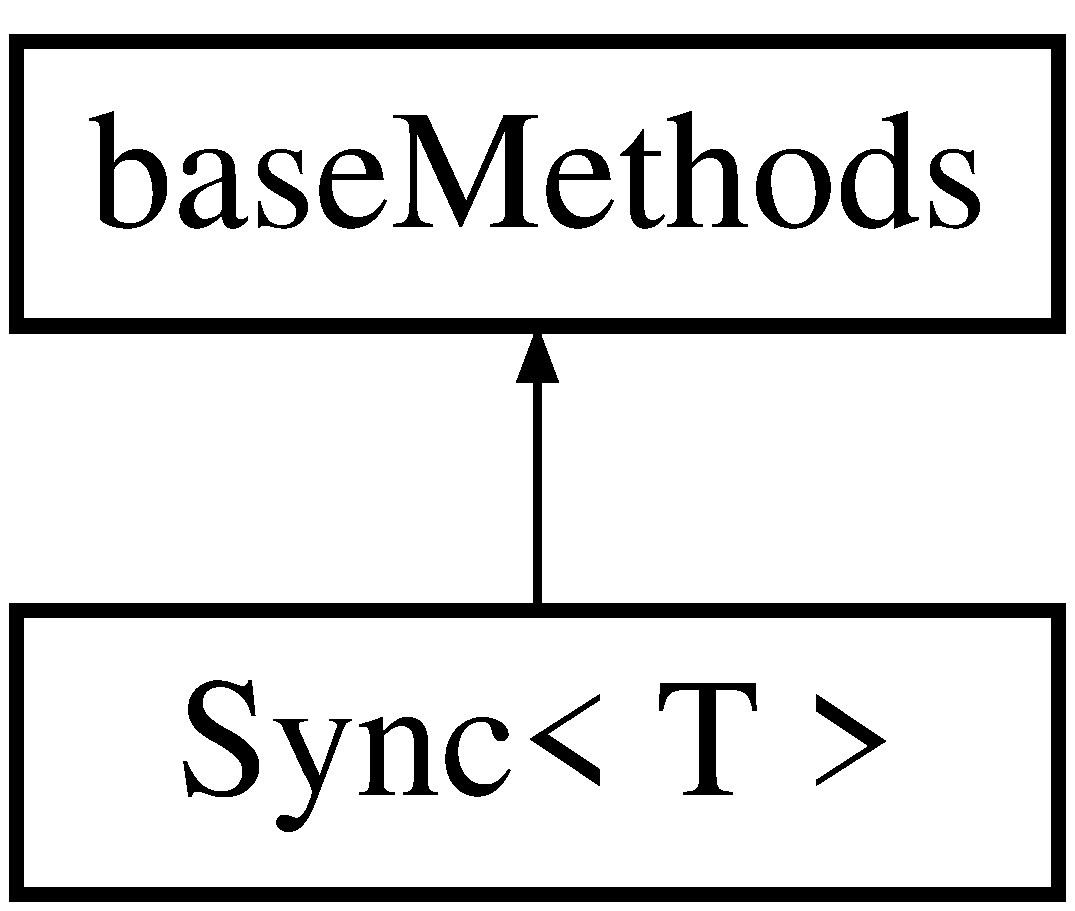
\includegraphics[height=2.000000cm]{class_sync}
\end{center}
\end{figure}
\subsection*{Public Types}
\begin{DoxyCompactItemize}
\item 
\mbox{\Hypertarget{class_sync_a84a754a69fe29401cc17a92e90c48975}\label{class_sync_a84a754a69fe29401cc17a92e90c48975}} 
typedef std\+::unique\+\_\+ptr$<$ T $>$ {\bfseries task\+Storage\+\_\+t}
\item 
\mbox{\Hypertarget{class_sync_a9b62760ba34279555be314fdc09a2690}\label{class_sync_a9b62760ba34279555be314fdc09a2690}} 
typedef \hyperlink{class_tasker_base}{Tasker\+Base} $\ast$ {\bfseries sub\+Task\+Storage\+\_\+t}
\item 
\mbox{\Hypertarget{class_sync_ae1688802d96c5882f89616a6fbf54fe7}\label{class_sync_ae1688802d96c5882f89616a6fbf54fe7}} 
typedef std\+::pair$<$ task\+Storage\+\_\+t, \hyperlink{class_tasker_base}{sub\+Task\+Storage\+\_\+t} $>$ {\bfseries task\+Pair\+Storage\+\_\+t}
\item 
\mbox{\Hypertarget{class_sync_a319cc5d12bb90918a33aea6aced00921}\label{class_sync_a319cc5d12bb90918a33aea6aced00921}} 
typedef std\+::list$<$ task\+Pair\+Storage\+\_\+t $>$ {\bfseries task\+List\+\_\+t}
\item 
\mbox{\Hypertarget{class_sync_a0d888c29e32980c1b54fcccf7a53e952}\label{class_sync_a0d888c29e32980c1b54fcccf7a53e952}} 
typedef std\+::function$<$ void(void)$>$ {\bfseries Empty\+Cb\+\_\+t}
\item 
\mbox{\Hypertarget{class_sync_a36eab6d1287f11d284de05b542afa3dc}\label{class_sync_a36eab6d1287f11d284de05b542afa3dc}} 
typedef std\+::function$<$ void(T \&)$>$ {\bfseries tasker\+Cb\+\_\+t}
\end{DoxyCompactItemize}
\subsection*{Public Member Functions}
\begin{DoxyCompactItemize}
\item 
\mbox{\Hypertarget{class_sync_aece81cdb63a55f8cbde87d19f6e3abb7}\label{class_sync_aece81cdb63a55f8cbde87d19f6e3abb7}} 
void {\bfseries loop} ()
\item 
\mbox{\Hypertarget{class_sync_a3fe1dc69eaf600a1cccdeb9a16ac9529}\label{class_sync_a3fe1dc69eaf600a1cccdeb9a16ac9529}} 
void {\bfseries enable} (bool enable)
\item 
\mbox{\Hypertarget{class_sync_a9e80ba41b50ccc48142210a178f01f1c}\label{class_sync_a9e80ba41b50ccc48142210a178f01f1c}} 
void {\bfseries set\+Repeat} (bool repeat)
\item 
\mbox{\Hypertarget{class_sync_a0bc032145bb002439b7af2a9611cc2e6}\label{class_sync_a0bc032145bb002439b7af2a9611cc2e6}} 
void {\bfseries sort} ()
\item 
\mbox{\Hypertarget{class_sync_aea43723f3a584a07137a47f50b40a9df}\label{class_sync_aea43723f3a584a07137a47f50b40a9df}} 
void {\bfseries dump\+Task} (T \&t, Stream \&stream, uint \&position, uint index)
\item 
\mbox{\Hypertarget{class_sync_af05b4166d049fdd643517980d090b232}\label{class_sync_af05b4166d049fdd643517980d090b232}} 
void {\bfseries printprechar} (Stream \&stream)
\end{DoxyCompactItemize}
\subsection*{Protected Attributes}
\begin{DoxyCompactItemize}
\item 
\mbox{\Hypertarget{class_sync_a257fec0e90c516a9d18f3f48e6dbc684}\label{class_sync_a257fec0e90c516a9d18f3f48e6dbc684}} 
task\+List\+\_\+t {\bfseries \+\_\+list}
\item 
\mbox{\Hypertarget{class_sync_ab238d6984e4942bbbf641a938ce109a1}\label{class_sync_ab238d6984e4942bbbf641a938ce109a1}} 
task\+List\+\_\+t\+::iterator {\bfseries \+\_\+it}
\end{DoxyCompactItemize}


The documentation for this class was generated from the following file\+:\begin{DoxyCompactItemize}
\item 
src/\+Tasker/src/\hyperlink{_task_methods_8h}{Task\+Methods.\+h}\end{DoxyCompactItemize}

\hypertarget{class_sys_log}{}\section{Sys\+Log Class Reference}
\label{class_sys_log}\index{Sys\+Log@{Sys\+Log}}
\subsection*{Public Member Functions}
\begin{DoxyCompactItemize}
\item 
\mbox{\Hypertarget{class_sys_log_a70bf3aae4dc469e141824bdc262df54e}\label{class_sys_log_a70bf3aae4dc469e141824bdc262df54e}} 
{\bfseries Sys\+Log} (I\+P\+Address ip, uint16\+\_\+t port, protocol\+\_\+t protocol=S\+Y\+S\+L\+O\+G\+\_\+\+P\+R\+O\+T\+O\+\_\+\+I\+E\+TF)
\item 
\mbox{\Hypertarget{class_sys_log_a070d1987bbdd7ee567e2fe8ca1fd6a2d}\label{class_sys_log_a070d1987bbdd7ee567e2fe8ca1fd6a2d}} 
void {\bfseries set\+Server} (I\+P\+Address ip, uint16\+\_\+t port)
\item 
\mbox{\Hypertarget{class_sys_log_ac1f59b46ba6d6ec34c5233ed872d1566}\label{class_sys_log_ac1f59b46ba6d6ec34c5233ed872d1566}} 
void {\bfseries set\+Mask} (uint8\+\_\+t mask)
\item 
\mbox{\Hypertarget{class_sys_log_ac7f2e2a2fad50db77251d4c642ba0279}\label{class_sys_log_ac7f2e2a2fad50db77251d4c642ba0279}} 
void {\bfseries set\+Priority} (uint16\+\_\+t priority)
\item 
\mbox{\Hypertarget{class_sys_log_a5255f07122744a41d827b0c5d14aed85}\label{class_sys_log_a5255f07122744a41d827b0c5d14aed85}} 
void {\bfseries set\+Device\+Name} (String name)
\item 
\mbox{\Hypertarget{class_sys_log_a60157e8bd07ef43fb0f75b8816b046b3}\label{class_sys_log_a60157e8bd07ef43fb0f75b8816b046b3}} 
void {\bfseries set\+App\+Name} (String \&name)
\item 
\mbox{\Hypertarget{class_sys_log_a61992419283847b0f4f2e240b6cd72e2}\label{class_sys_log_a61992419283847b0f4f2e240b6cd72e2}} 
void {\bfseries set\+Protocol} (protocol\+\_\+t protocol)
\item 
\mbox{\Hypertarget{class_sys_log_a3b245553018d0e04f1943e284beb6a58}\label{class_sys_log_a3b245553018d0e04f1943e284beb6a58}} 
bool {\bfseries log} (\hyperlink{class_e_s_p_m_a_n_1_1my_string}{my\+String} msg)
\item 
\mbox{\Hypertarget{class_sys_log_a567695ffcfc39e65f3c2121949e764d2}\label{class_sys_log_a567695ffcfc39e65f3c2121949e764d2}} 
bool {\bfseries log} (uint16\+\_\+t pri, \hyperlink{class_e_s_p_m_a_n_1_1my_string}{my\+String} msg)
\item 
\mbox{\Hypertarget{class_sys_log_a1a6053509377113ecc7653d4298803a9}\label{class_sys_log_a1a6053509377113ecc7653d4298803a9}} 
bool {\bfseries log} (\hyperlink{class_e_s_p_m_a_n_1_1my_string}{my\+String} app\+Name, \hyperlink{class_e_s_p_m_a_n_1_1my_string}{my\+String} msg)
\item 
\mbox{\Hypertarget{class_sys_log_a151d2992fdc2a6ea0a52996e34a4a21f}\label{class_sys_log_a151d2992fdc2a6ea0a52996e34a4a21f}} 
bool {\bfseries log} (uint16\+\_\+t pri, \hyperlink{class_e_s_p_m_a_n_1_1my_string}{my\+String} app\+Name, \hyperlink{class_e_s_p_m_a_n_1_1my_string}{my\+String} msg)
\end{DoxyCompactItemize}


The documentation for this class was generated from the following files\+:\begin{DoxyCompactItemize}
\item 
src/\hyperlink{_e_s_pman_sys_log_8h}{E\+S\+Pman\+Sys\+Log.\+h}\item 
src/\hyperlink{_e_s_pman_sys_log_8cpp}{E\+S\+Pman\+Sys\+Log.\+cpp}\end{DoxyCompactItemize}

\hypertarget{class_task}{}\section{Task Class Reference}
\label{class_task}\index{Task@{Task}}
\subsection*{Public Types}
\begin{DoxyCompactItemize}
\item 
\mbox{\Hypertarget{class_task_a3c14c4e1c42ebd30ba57a1d6da0d74bb}\label{class_task_a3c14c4e1c42ebd30ba57a1d6da0d74bb}} 
typedef std\+::function$<$ void(\hyperlink{class_task}{Task} \&)$>$ {\bfseries tasker\+Cb\+\_\+t}
\end{DoxyCompactItemize}
\subsection*{Public Member Functions}
\begin{DoxyCompactItemize}
\item 
\mbox{\Hypertarget{class_task_abf4c9149babce0960cf1e628de499f9d}\label{class_task_abf4c9149babce0960cf1e628de499f9d}} 
{\bfseries Task} (tasker\+Cb\+\_\+t cb, bool use\+Micros=false)
\item 
\mbox{\Hypertarget{class_task_ab69f69089f91b6b7c696564a6796e0ca}\label{class_task_ab69f69089f91b6b7c696564a6796e0ca}} 
bool {\bfseries run} (const uint8\+\_\+t priority=0, const bool override=false)
\item 
\mbox{\Hypertarget{class_task_a1fc4c9c46651e9c4fc0240b5619ea850}\label{class_task_a1fc4c9c46651e9c4fc0240b5619ea850}} 
\hyperlink{class_task}{Task} \& {\bfseries run\+Cb} ()
\item 
\mbox{\Hypertarget{class_task_ae65879becb23f5381225ee0c8959b739}\label{class_task_ae65879becb23f5381225ee0c8959b739}} 
\hyperlink{class_task}{Task} \& {\bfseries set\+Timeout} (uint32\+\_\+t timeout)
\item 
\mbox{\Hypertarget{class_task_a602c3d55c3ce1adf70c77ca34dac5eba}\label{class_task_a602c3d55c3ce1adf70c77ca34dac5eba}} 
uint32\+\_\+t {\bfseries get\+Timeout} ()
\item 
\mbox{\Hypertarget{class_task_af0cdd7eb17b54decbca227cc2db86aaa}\label{class_task_af0cdd7eb17b54decbca227cc2db86aaa}} 
\hyperlink{class_task}{Task} \& {\bfseries set\+Repeat} (bool repeat=true)
\item 
\mbox{\Hypertarget{class_task_a2eba537a294f1ea2e9d0d375ad980993}\label{class_task_a2eba537a294f1ea2e9d0d375ad980993}} 
\hyperlink{class_task}{Task} \& {\bfseries set\+Repeat} (int number)
\item 
\mbox{\Hypertarget{class_task_aed0f55a2f6129e1ee9ec6bf1f49339ba}\label{class_task_aed0f55a2f6129e1ee9ec6bf1f49339ba}} 
\hyperlink{class_task}{Task} \& {\bfseries set\+Priority} (uint8\+\_\+t pr)
\item 
\mbox{\Hypertarget{class_task_affea110babfe474fc6ccdb88e7b8122e}\label{class_task_affea110babfe474fc6ccdb88e7b8122e}} 
uint8\+\_\+t {\bfseries get\+Priority} ()
\item 
\mbox{\Hypertarget{class_task_a7f9a1b3b8b2f16bba8fa05831dff6776}\label{class_task_a7f9a1b3b8b2f16bba8fa05831dff6776}} 
\hyperlink{class_task}{Task} \& {\bfseries enable} ()
\item 
\mbox{\Hypertarget{class_task_afe347b4ccfcaf48c333f87cd4e832ecf}\label{class_task_afe347b4ccfcaf48c333f87cd4e832ecf}} 
\hyperlink{class_task}{Task} \& {\bfseries disable} ()
\item 
\mbox{\Hypertarget{class_task_ab3d1be80ad209a597a729166a80efc92}\label{class_task_ab3d1be80ad209a597a729166a80efc92}} 
\hyperlink{class_task}{Task} \& {\bfseries set\+Name} (const char $\ast$name)
\item 
\mbox{\Hypertarget{class_task_aba0bd15f206791e57958128c5be34956}\label{class_task_aba0bd15f206791e57958128c5be34956}} 
const char $\ast$ {\bfseries name} ()
\item 
\mbox{\Hypertarget{class_task_aa3a2b2bf899730aa64e1cf3c1d868b47}\label{class_task_aa3a2b2bf899730aa64e1cf3c1d868b47}} 
void {\bfseries reset} ()
\item 
\mbox{\Hypertarget{class_task_a4804088579cabf62cd81f2f85d79f5c4}\label{class_task_a4804088579cabf62cd81f2f85d79f5c4}} 
\hyperlink{class_task}{Task} \& {\bfseries on\+End} (std\+::function$<$ void(void)$>$ Cb)
\item 
\mbox{\Hypertarget{class_task_a60541f7f451ab3ce1831530272e1d428}\label{class_task_a60541f7f451ab3ce1831530272e1d428}} 
\hyperlink{class_task}{Task} \& {\bfseries set\+Persistent} (bool donotdelete)
\item 
\mbox{\Hypertarget{class_task_a0922035b69fa2db9fcfc8624e0857724}\label{class_task_a0922035b69fa2db9fcfc8624e0857724}} 
bool {\bfseries running} ()
\end{DoxyCompactItemize}
\subsection*{Public Attributes}
\begin{DoxyCompactItemize}
\item 
\mbox{\Hypertarget{class_task_a658d28d140840da2ae4ea5a92923a326}\label{class_task_a658d28d140840da2ae4ea5a92923a326}} 
uint32\+\_\+t {\bfseries count} \{0\}
\end{DoxyCompactItemize}


The documentation for this class was generated from the following file\+:\begin{DoxyCompactItemize}
\item 
src/\+Tasker/src/\hyperlink{_task_8h}{Task.\+h}\end{DoxyCompactItemize}

\hypertarget{class_tasker}{}\section{Tasker$<$ Task\+Type, Loop\+Method $>$ Class Template Reference}
\label{class_tasker}\index{Tasker$<$ Task\+Type, Loop\+Method $>$@{Tasker$<$ Task\+Type, Loop\+Method $>$}}
Inheritance diagram for Tasker$<$ Task\+Type, Loop\+Method $>$\+:\begin{figure}[H]
\begin{center}
\leavevmode
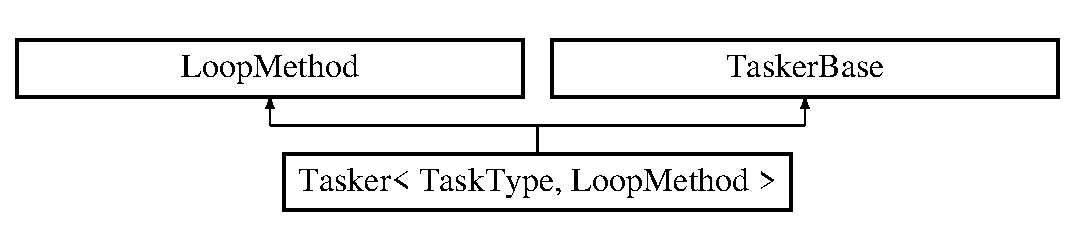
\includegraphics[height=2.000000cm]{class_tasker}
\end{center}
\end{figure}
\subsection*{Public Types}
\begin{DoxyCompactItemize}
\item 
\mbox{\Hypertarget{class_tasker_a3e9340a4891ee26049746f6a37fa1d65}\label{class_tasker_a3e9340a4891ee26049746f6a37fa1d65}} 
typedef Loop\+Method {\bfseries loop\+\_\+m}
\item 
\mbox{\Hypertarget{class_tasker_ace2643f69a2c9298541577a25178d6cf}\label{class_tasker_ace2643f69a2c9298541577a25178d6cf}} 
typedef Task\+Type {\bfseries task\+\_\+t}
\end{DoxyCompactItemize}
\subsection*{Public Member Functions}
\begin{DoxyCompactItemize}
\item 
\mbox{\Hypertarget{class_tasker_ab1b011929f82e45e6de96be3ad816680}\label{class_tasker_ab1b011929f82e45e6de96be3ad816680}} 
Task\+Type \& {\bfseries add} (tasker\+Cb\+\_\+t Cb, bool use\+Micros=false)
\item 
\mbox{\Hypertarget{class_tasker_a8823e80ee99db02faf92e800c1a0189c}\label{class_tasker_a8823e80ee99db02faf92e800c1a0189c}} 
Task\+Type \& {\bfseries add\+Before} (tasker\+Cb\+\_\+t Cb, bool use\+Micros=false)
\item 
\mbox{\Hypertarget{class_tasker_a82d870310017354b4a7185fedcd74a08}\label{class_tasker_a82d870310017354b4a7185fedcd74a08}} 
Task\+Type \& {\bfseries add\+After} (tasker\+Cb\+\_\+t Cb, bool use\+Micros=false)
\item 
\mbox{\Hypertarget{class_tasker_a2b1027cad18c0b510c252c78e07cd23e}\label{class_tasker_a2b1027cad18c0b510c252c78e07cd23e}} 
bool {\bfseries go\+To\+Task} (Task\+Type \&task, bool run\+Immediately=false)
\item 
\mbox{\Hypertarget{class_tasker_ac04ba2b621aaf631fa0bcffb429dbcda}\label{class_tasker_ac04ba2b621aaf631fa0bcffb429dbcda}} 
bool {\bfseries remove} (Task\+Type \&task)
\item 
\mbox{\Hypertarget{class_tasker_af9f0f1b6152e21adb2075d29890365d3}\label{class_tasker_af9f0f1b6152e21adb2075d29890365d3}} 
void {\bfseries debug\+Out} (Stream \&stream, uint index\+Num=0, uint position=0)
\item 
\mbox{\Hypertarget{class_tasker_a9bc456b890c556f028f27d0ce85507e8}\label{class_tasker_a9bc456b890c556f028f27d0ce85507e8}} 
{\footnotesize template$<$class Tasker\+Type $>$ }\\Tasker\+Type $\ast$ {\bfseries add\+Sub\+Tasker} (bool do\+Not\+Delete=false)
\item 
\mbox{\Hypertarget{class_tasker_ac243549b2515839aae51a1b818611e14}\label{class_tasker_ac243549b2515839aae51a1b818611e14}} 
bool {\bfseries is\+Empty} ()
\item 
\mbox{\Hypertarget{class_tasker_a55d556448981dd30f79056c6a5eebc9a}\label{class_tasker_a55d556448981dd30f79056c6a5eebc9a}} 
void {\bfseries test} ()
\item 
\mbox{\Hypertarget{class_tasker_ae2b2459b894cd113d57a417963fe1ec9}\label{class_tasker_ae2b2459b894cd113d57a417963fe1ec9}} 
void {\bfseries set\+Parent} (\hyperlink{class_tasker_base}{Tasker\+Base} $\ast$ptr)
\end{DoxyCompactItemize}


The documentation for this class was generated from the following file\+:\begin{DoxyCompactItemize}
\item 
src/\+Tasker/src/\hyperlink{_tasker_class_8h}{Tasker\+Class.\+h}\end{DoxyCompactItemize}

\hypertarget{class_tasker_base}{}\section{Tasker\+Base Class Reference}
\label{class_tasker_base}\index{Tasker\+Base@{Tasker\+Base}}
Inheritance diagram for Tasker\+Base\+:\begin{figure}[H]
\begin{center}
\leavevmode
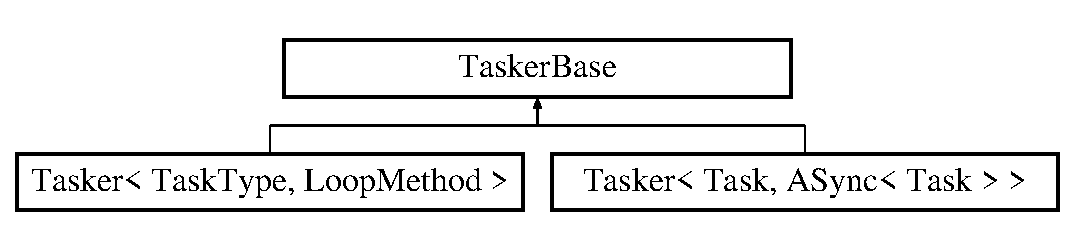
\includegraphics[height=2.000000cm]{class_tasker_base}
\end{center}
\end{figure}
\subsection*{Public Member Functions}
\begin{DoxyCompactItemize}
\item 
\mbox{\Hypertarget{class_tasker_base_a7bf4774e6d8cf33fb5ce54e5ff6abfac}\label{class_tasker_base_a7bf4774e6d8cf33fb5ce54e5ff6abfac}} 
virtual void {\bfseries debug\+Out} (Stream \&stream, uint index\+Num=0, uint indentlevel=0)
\item 
\mbox{\Hypertarget{class_tasker_base_a9da41046397c54692d9067203f761923}\label{class_tasker_base_a9da41046397c54692d9067203f761923}} 
virtual void {\bfseries test} ()
\end{DoxyCompactItemize}


The documentation for this class was generated from the following file\+:\begin{DoxyCompactItemize}
\item 
src/\+Tasker/src/\hyperlink{_tasker_class_8h}{Tasker\+Class.\+h}\end{DoxyCompactItemize}

\hypertarget{struct_e_s_pdevice_finder_1_1_u_d_p__item}{}\section{E\+S\+Pdevice\+Finder\+:\+:U\+D\+P\+\_\+item Struct Reference}
\label{struct_e_s_pdevice_finder_1_1_u_d_p__item}\index{E\+S\+Pdevice\+Finder\+::\+U\+D\+P\+\_\+item@{E\+S\+Pdevice\+Finder\+::\+U\+D\+P\+\_\+item}}
\subsection*{Public Member Functions}
\begin{DoxyCompactItemize}
\item 
\mbox{\Hypertarget{struct_e_s_pdevice_finder_1_1_u_d_p__item_a260d0a61d7782a6d8ba0a1d146a71ce1}\label{struct_e_s_pdevice_finder_1_1_u_d_p__item_a260d0a61d7782a6d8ba0a1d146a71ce1}} 
{\bfseries U\+D\+P\+\_\+item} (I\+P\+Address ip, std\+::unique\+\_\+ptr$<$ char\mbox{[}$\,$\mbox{]}$>$(ID))
\end{DoxyCompactItemize}
\subsection*{Public Attributes}
\begin{DoxyCompactItemize}
\item 
\mbox{\Hypertarget{struct_e_s_pdevice_finder_1_1_u_d_p__item_a55a4344f5414301dd6acea63982c1771}\label{struct_e_s_pdevice_finder_1_1_u_d_p__item_a55a4344f5414301dd6acea63982c1771}} 
I\+P\+Address {\bfseries IP}
\item 
\mbox{\Hypertarget{struct_e_s_pdevice_finder_1_1_u_d_p__item_a25937016f1387c66de6fc1310ddf006d}\label{struct_e_s_pdevice_finder_1_1_u_d_p__item_a25937016f1387c66de6fc1310ddf006d}} 
std\+::unique\+\_\+ptr$<$ char\mbox{[}$\,$\mbox{]}$>$ {\bfseries name}
\item 
\mbox{\Hypertarget{struct_e_s_pdevice_finder_1_1_u_d_p__item_a2f68508a0b6d46ca91e1354f9de52cfc}\label{struct_e_s_pdevice_finder_1_1_u_d_p__item_a2f68508a0b6d46ca91e1354f9de52cfc}} 
uint32\+\_\+t {\bfseries lastseen} \{0\}
\end{DoxyCompactItemize}


The documentation for this struct was generated from the following files\+:\begin{DoxyCompactItemize}
\item 
src/\+E\+S\+Pdevice\+Finder/src/E\+S\+Pdevice\+Finder.\+h\item 
src/\+E\+S\+Pdevice\+Finder/src/E\+S\+Pdevice\+Finder.\+cpp\end{DoxyCompactItemize}

\chapter{File Documentation}
\hypertarget{_e_s_p_m_a_n_8cpp}{}\section{src/\+E\+S\+P\+M\+AN.cpp File Reference}
\label{_e_s_p_m_a_n_8cpp}\index{src/\+E\+S\+P\+M\+A\+N.\+cpp@{src/\+E\+S\+P\+M\+A\+N.\+cpp}}


E\+S\+P\+M\+AN file.  


{\ttfamily \#include \char`\"{}E\+S\+P\+M\+A\+N.\+h\char`\"{}}\newline


\subsection{Detailed Description}
E\+S\+P\+M\+AN file. 

Details. 
\hypertarget{_e_s_p_m_a_n_8h}{}\section{src/\+E\+S\+P\+M\+AN.h File Reference}
\label{_e_s_p_m_a_n_8h}\index{src/\+E\+S\+P\+M\+A\+N.\+h@{src/\+E\+S\+P\+M\+A\+N.\+h}}


E\+S\+P\+M\+AN file.  


{\ttfamily \#include $<$Arduino.\+h$>$}\newline
{\ttfamily \#include $<$Arduino\+Json.\+h$>$}\newline
{\ttfamily \#include $<$I\+P\+Address.\+h$>$}\newline
{\ttfamily \#include $<$functional$>$}\newline
{\ttfamily \#include $<$F\+S.\+h$>$}\newline
\subsection*{Classes}
\begin{DoxyCompactItemize}
\item 
class \hyperlink{class_e_s_p_m_a_n_1_1_j_s_o_npackage}{E\+S\+P\+M\+A\+N\+::\+J\+S\+O\+Npackage}
\item 
class \hyperlink{class_e_s_p_m_a_n_1_1my_string}{E\+S\+P\+M\+A\+N\+::my\+String}
\item 
class \hyperlink{class_e_s_p_m_a_n_1_1my_stringf}{E\+S\+P\+M\+A\+N\+::my\+Stringf}
\item 
class \hyperlink{class_e_s_p_m_a_n_1_1my_stringf___p}{E\+S\+P\+M\+A\+N\+::my\+Stringf\+\_\+P}
\item 
struct \hyperlink{struct_e_s_p_m_a_n_1_1settings__t}{E\+S\+P\+M\+A\+N\+::settings\+\_\+t}
\item 
struct \hyperlink{struct_e_s_p_m_a_n_1_1settings__t_1_1_a_p__t}{E\+S\+P\+M\+A\+N\+::settings\+\_\+t\+::\+A\+P\+\_\+t}
\item 
struct \hyperlink{struct_e_s_p_m_a_n_1_1settings__t_1_1_s_t_a__t}{E\+S\+P\+M\+A\+N\+::settings\+\_\+t\+::\+S\+T\+A\+\_\+t}
\item 
struct \hyperlink{struct_e_s_p_m_a_n_1_1settings__t_1_1_g_e_n__t}{E\+S\+P\+M\+A\+N\+::settings\+\_\+t\+::\+G\+E\+N\+\_\+t}
\item 
struct \hyperlink{struct_e_s_p_m_a_n_1_1password__t}{E\+S\+P\+M\+A\+N\+::password\+\_\+t}
\end{DoxyCompactItemize}
\subsection*{Enumerations}
\begin{DoxyCompactItemize}
\item 
\mbox{\Hypertarget{_e_s_p_m_a_n_8h_a8bcc85d695e1fff66ea9b0abf4891a78}\label{_e_s_p_m_a_n_8h_a8bcc85d695e1fff66ea9b0abf4891a78}} 
enum {\bfseries E\+S\+P\+M\+A\+N\+\_\+\+E\+R\+R\+\_\+t} \+: int8\+\_\+t \{ \newline
{\bfseries S\+U\+C\+C\+E\+SS} = 0, 
{\bfseries U\+N\+K\+N\+O\+W\+N\+\_\+\+E\+R\+R\+OR} = -\/20, 
{\bfseries N\+O\+\_\+\+U\+P\+D\+A\+T\+E\+\_\+\+U\+RL} = -\/21, 
{\bfseries S\+P\+I\+F\+F\+S\+\_\+\+F\+I\+L\+E\+S\+\_\+\+A\+B\+S\+E\+NT} = -\/22, 
\newline
{\bfseries F\+I\+L\+E\+\_\+\+N\+O\+T\+\_\+\+C\+H\+A\+N\+G\+ED} = -\/23, 
{\bfseries M\+D5\+\_\+\+C\+H\+K\+\_\+\+E\+R\+R\+OR} = -\/24, 
{\bfseries H\+T\+T\+P\+\_\+\+E\+R\+R\+OR} = -\/25, 
{\bfseries J\+S\+O\+N\+\_\+\+P\+A\+R\+S\+E\+\_\+\+E\+R\+R\+OR} = -\/26, 
\newline
{\bfseries J\+S\+O\+N\+\_\+\+O\+B\+J\+E\+C\+T\+\_\+\+E\+R\+R\+OR} = -\/27, 
{\bfseries C\+O\+N\+F\+I\+G\+\_\+\+F\+I\+L\+E\+\_\+\+E\+R\+R\+OR} = -\/28, 
{\bfseries U\+P\+D\+A\+T\+E\+R\+\_\+\+E\+R\+R\+OR} = -\/29, 
{\bfseries J\+S\+O\+N\+\_\+\+T\+O\+O\+\_\+\+L\+A\+R\+GE} = -\/30, 
\newline
{\bfseries M\+A\+L\+L\+O\+C\+\_\+\+F\+A\+IL} = -\/31, 
{\bfseries M\+A\+N\+I\+F\+S\+T\+\_\+\+F\+I\+L\+E\+\_\+\+E\+R\+R\+OR} = -\/32, 
{\bfseries U\+N\+K\+N\+O\+W\+N\+\_\+\+N\+U\+M\+B\+E\+R\+\_\+\+O\+F\+\_\+\+F\+I\+L\+ES} = -\/33, 
{\bfseries S\+P\+I\+F\+F\+S\+\_\+\+I\+N\+F\+O\+\_\+\+F\+A\+IL} = -\/34, 
\newline
{\bfseries S\+P\+I\+F\+F\+S\+\_\+\+F\+I\+L\+E\+N\+A\+M\+E\+\_\+\+T\+O\+O\+\_\+\+L\+O\+NG} = -\/35, 
{\bfseries S\+P\+I\+F\+F\+S\+\_\+\+F\+I\+L\+E\+\_\+\+O\+P\+E\+N\+\_\+\+E\+R\+R\+OR} = -\/36, 
{\bfseries F\+I\+L\+E\+\_\+\+T\+O\+O\+\_\+\+L\+A\+R\+GE} = -\/37, 
{\bfseries I\+N\+C\+O\+M\+P\+L\+E\+T\+E\+\_\+\+D\+O\+W\+N\+L\+O\+AD} = -\/38, 
\newline
{\bfseries C\+R\+C\+\_\+\+E\+R\+R\+OR} = -\/39, 
{\bfseries J\+S\+O\+N\+\_\+\+K\+E\+Y\+\_\+\+M\+I\+S\+S\+I\+NG} = -\/40, 
{\bfseries E\+M\+P\+T\+Y\+\_\+\+B\+U\+F\+F\+ER} = -\/41, 
{\bfseries A\+P\+\_\+\+D\+I\+S\+A\+B\+L\+ED} = -\/42, 
\newline
{\bfseries E\+R\+R\+O\+R\+\_\+\+E\+N\+A\+B\+L\+I\+N\+G\+\_\+\+AP} = -\/43, 
{\bfseries E\+R\+R\+O\+R\+\_\+\+D\+I\+S\+A\+B\+L\+I\+N\+G\+\_\+\+AP} = -\/44, 
{\bfseries E\+R\+R\+O\+R\+\_\+\+S\+E\+T\+T\+I\+N\+G\+\_\+\+C\+O\+N\+F\+IG} = -\/45, 
{\bfseries E\+R\+R\+O\+R\+\_\+\+E\+N\+A\+B\+L\+I\+N\+G\+\_\+\+S\+TA} = -\/46, 
\newline
{\bfseries F\+A\+I\+L\+E\+D\+\_\+\+S\+E\+T\+\_\+\+A\+U\+T\+O\+C\+O\+N\+N\+E\+CT} = -\/47, 
{\bfseries F\+A\+I\+L\+E\+D\+\_\+\+S\+E\+T\+\_\+\+A\+U\+T\+O\+R\+E\+C\+O\+N\+N\+E\+CT} = -\/48, 
{\bfseries W\+I\+F\+I\+\_\+\+C\+O\+N\+F\+I\+G\+\_\+\+E\+R\+R\+OR} = -\/49, 
{\bfseries N\+O\+\_\+\+S\+T\+A\+\_\+\+S\+S\+ID} = -\/50, 
\newline
{\bfseries E\+R\+R\+O\+R\+\_\+\+W\+I\+F\+I\+\_\+\+B\+E\+G\+IN} = -\/60, 
{\bfseries N\+O\+\_\+\+S\+S\+I\+D\+\_\+\+A\+V\+A\+IL} = -\/70, 
{\bfseries C\+O\+N\+N\+E\+C\+T\+\_\+\+F\+A\+I\+L\+ED} = -\/80, 
{\bfseries U\+N\+I\+T\+I\+T\+I\+A\+L\+I\+S\+ED} = -\/81, 
\newline
{\bfseries E\+R\+R\+O\+R\+\_\+\+S\+P\+I\+F\+F\+S\+\_\+\+M\+O\+U\+NT} = -\/82, 
{\bfseries A\+U\+T\+O\+\_\+\+C\+O\+N\+N\+E\+C\+T\+E\+D\+\_\+\+S\+TA} = -\/83, 
{\bfseries E\+R\+R\+O\+R\+\_\+\+D\+I\+S\+A\+B\+L\+I\+N\+G\+\_\+\+S\+TA} = -\/84, 
{\bfseries S\+T\+A\+\_\+\+D\+I\+S\+A\+B\+L\+ED} = -\/85, 
\newline
{\bfseries S\+E\+T\+T\+I\+N\+G\+S\+\_\+\+N\+O\+T\+\_\+\+I\+N\+\_\+\+M\+E\+M\+O\+RY} = -\/86, 
{\bfseries E\+R\+R\+O\+R\+\_\+\+S\+E\+T\+T\+I\+N\+G\+\_\+\+M\+AC} = -\/87, 
{\bfseries P\+A\+S\+S\+W\+O\+R\+D\+\_\+\+M\+I\+S\+M\+A\+T\+CH} = -\/88, 
{\bfseries N\+O\+\_\+\+C\+H\+A\+N\+G\+ES} = -\/89, 
\newline
{\bfseries P\+A\+S\+S\+W\+O\+R\+O\+D\+\_\+\+I\+N\+V\+A\+L\+ID} = -\/90, 
{\bfseries W\+R\+O\+N\+G\+\_\+\+S\+E\+T\+T\+I\+N\+G\+S\+\_\+\+F\+I\+L\+E\+\_\+\+V\+E\+R\+S\+I\+ON} = -\/91
 \}
\item 
\mbox{\Hypertarget{_e_s_p_m_a_n_8h_a367257b39aefb98c08769d372c069820}\label{_e_s_p_m_a_n_8h_a367257b39aefb98c08769d372c069820}} 
enum {\bfseries ap\+\_\+boot\+\_\+mode\+\_\+t} \+: int8\+\_\+t \{ \newline
{\bfseries D\+I\+S\+A\+B\+L\+ED} = -\/1, 
{\bfseries N\+O\+\_\+\+S\+T\+A\+\_\+\+B\+O\+OT} = 0, 
{\bfseries N\+O\+\_\+\+S\+T\+A\+\_\+\+B\+O\+O\+T\+\_\+\+A\+P\+\_\+5} = 5, 
{\bfseries N\+O\+\_\+\+S\+T\+A\+\_\+\+B\+O\+O\+T\+\_\+\+A\+P\+\_\+10} = 10, 
\newline
{\bfseries N\+O\+\_\+\+S\+T\+A\+\_\+\+B\+O\+O\+T\+\_\+\+A\+P\+\_\+30} = 30, 
{\bfseries N\+O\+\_\+\+S\+T\+A\+\_\+\+B\+O\+O\+T\+\_\+\+A\+P\+\_\+60} = 60
 \}
\item 
\mbox{\Hypertarget{_e_s_p_m_a_n_8h_a48ab5fdcc0f24c796c52b63426135429}\label{_e_s_p_m_a_n_8h_a48ab5fdcc0f24c796c52b63426135429}} 
enum {\bfseries no\+\_\+sta\+\_\+mode\+\_\+t} \+: int8\+\_\+t \{ \newline
{\bfseries N\+O\+\_\+\+S\+T\+A\+\_\+\+N\+O\+T\+H\+I\+NG} = -\/2, 
{\bfseries N\+O\+\_\+\+S\+T\+A\+\_\+\+R\+E\+B\+O\+OT} = -\/1, 
{\bfseries N\+O\+\_\+\+S\+T\+A\+\_\+\+S\+T\+A\+R\+T\+\_\+\+AP} = 0, 
{\bfseries N\+O\+\_\+\+S\+T\+A\+\_\+\+S\+T\+A\+R\+T\+\_\+\+A\+P\+\_\+5} = 5, 
\newline
{\bfseries N\+O\+\_\+\+S\+T\+A\+\_\+\+S\+T\+A\+R\+T\+\_\+\+A\+P\+\_\+10} = 10, 
{\bfseries N\+O\+\_\+\+S\+T\+A\+\_\+\+S\+T\+A\+R\+T\+\_\+\+A\+P\+\_\+30} = 30, 
{\bfseries N\+O\+\_\+\+S\+T\+A\+\_\+\+S\+T\+A\+R\+T\+\_\+\+A\+P\+\_\+60} = 60
 \}
\end{DoxyCompactItemize}
\subsection*{Variables}
\begin{DoxyCompactItemize}
\item 
\mbox{\Hypertarget{_e_s_p_m_a_n_8h_aa88c03e5f6478d3ce6c6e9537c83f8a8}\label{_e_s_p_m_a_n_8h_aa88c03e5f6478d3ce6c6e9537c83f8a8}} 
const char fstring\+\_\+\+C\+O\+RS \mbox{[}$\,$\mbox{]} {\bfseries E\+S\+P\+M\+A\+N\+::\+P\+R\+O\+G\+M\+EM} = \char`\"{}Access-\/Control-\/Allow-\/Origin\char`\"{}
\end{DoxyCompactItemize}


\subsection{Detailed Description}
E\+S\+P\+M\+AN file. 

Details. 
\hypertarget{_e_s_pmanager_8cpp}{}\section{src/\+E\+S\+Pmanager.cpp File Reference}
\label{_e_s_pmanager_8cpp}\index{src/\+E\+S\+Pmanager.\+cpp@{src/\+E\+S\+Pmanager.\+cpp}}


\hyperlink{class_e_s_pmanager}{E\+S\+Pmanager} file.  


{\ttfamily \#include \char`\"{}E\+S\+Pmanager.\+h\char`\"{}}\newline
{\ttfamily \#include $<$Wi\+Fi\+Udp.\+h$>$}\newline
{\ttfamily \#include $<$Arduino\+O\+T\+A.\+h$>$}\newline
{\ttfamily \#include $<$flash\+\_\+utils.\+h$>$}\newline
{\ttfamily \#include $<$Arduino\+Json.\+h$>$}\newline
{\ttfamily \#include $<$E\+S\+P8266m\+D\+N\+S.\+h$>$}\newline
{\ttfamily \#include $<$M\+D5\+Builder.\+h$>$}\newline
{\ttfamily \#include $<$Async\+Json.\+h$>$}\newline
{\ttfamily \#include $<$umm\+\_\+malloc/umm\+\_\+malloc.\+h$>$}\newline
{\ttfamily \#include $<$time.\+h$>$}\newline
{\ttfamily \#include $<$stdio.\+h$>$}\newline
{\ttfamily \#include $<$Web\+Authentication.\+h$>$}\newline
{\ttfamily \#include $<$Hash.\+h$>$}\newline
{\ttfamily \#include $<$list$>$}\newline
{\ttfamily \#include \char`\"{}Tasker/src/\+Tasker.\+h\char`\"{}}\newline
{\ttfamily \#include \char`\"{}Flash\+Writer.\+h\char`\"{}}\newline
{\ttfamily \#include \char`\"{}user\+\_\+interface.\+h\char`\"{}}\newline
\subsection*{Macros}
\begin{DoxyCompactItemize}
\item 
\mbox{\Hypertarget{_e_s_pmanager_8cpp_afa047aa3ce412a43c328eb9527433818}\label{_e_s_pmanager_8cpp_afa047aa3ce412a43c328eb9527433818}} 
\#define {\bfseries E\+S\+P\+M\+A\+N\+A\+G\+E\+R\+\_\+\+G\+I\+T\+\_\+\+T\+AG}~\char`\"{}N\+OT D\+E\+F\+I\+N\+ED\char`\"{}
\end{DoxyCompactItemize}
\subsection*{Variables}
\begin{DoxyCompactItemize}
\item 
\mbox{\Hypertarget{_e_s_pmanager_8cpp_af943fe6ef5c41707adbf4c6c56448165}\label{_e_s_pmanager_8cpp_af943fe6ef5c41707adbf4c6c56448165}} 
U\+M\+M\+\_\+\+H\+E\+A\+P\+\_\+\+I\+N\+FO {\bfseries umm\+Heap\+Info}
\item 
\mbox{\Hypertarget{_e_s_pmanager_8cpp_a39217f4a317d9376abd1434c535576db}\label{_e_s_pmanager_8cpp_a39217f4a317d9376abd1434c535576db}} 
uint32\+\_\+t {\bfseries \+\_\+\+S\+P\+I\+F\+F\+S\+\_\+start}
\end{DoxyCompactItemize}


\subsection{Detailed Description}
\hyperlink{class_e_s_pmanager}{E\+S\+Pmanager} file. 

Details. 
\hypertarget{_e_s_pmanager_8h}{}\section{src/\+E\+S\+Pmanager.h File Reference}
\label{_e_s_pmanager_8h}\index{src/\+E\+S\+Pmanager.\+h@{src/\+E\+S\+Pmanager.\+h}}


\hyperlink{class_e_s_pmanager}{E\+S\+Pmanager} file.  


{\ttfamily \#include $<$Arduino.\+h$>$}\newline
{\ttfamily \#include $<$E\+S\+P8266\+Wi\+Fi.\+h$>$}\newline
{\ttfamily \#include $<$E\+S\+P\+Async\+T\+C\+P.\+h$>$}\newline
{\ttfamily \#include $<$E\+S\+P\+Async\+Web\+Server.\+h$>$}\newline
{\ttfamily \#include $<$E\+S\+P8266\+H\+T\+T\+P\+Client.\+h$>$}\newline
{\ttfamily \#include $<$E\+S\+P8266http\+Update.\+h$>$}\newline
{\ttfamily \#include $<$D\+N\+S\+Server.\+h$>$}\newline
{\ttfamily \#include $<$F\+S.\+h$>$}\newline
{\ttfamily \#include $<$functional$>$}\newline
{\ttfamily \#include $<$Arduino\+Json.\+h$>$}\newline
{\ttfamily \#include \char`\"{}Tasker/src/\+Tasker.\+h\char`\"{}}\newline
{\ttfamily \#include \char`\"{}E\+S\+Pdevice\+Finder/src/\+E\+S\+Pdevice\+Finder.\+h\char`\"{}}\newline
{\ttfamily \#include \char`\"{}E\+S\+P\+M\+A\+N.\+h\char`\"{}}\newline
{\ttfamily \#include $<$E\+S\+Pman\+Sys\+Log.\+h$>$}\newline
\subsection*{Classes}
\begin{DoxyCompactItemize}
\item 
class \hyperlink{class_e_s_pmanager}{E\+S\+Pmanager}
\end{DoxyCompactItemize}
\subsection*{Macros}
\begin{DoxyCompactItemize}
\item 
\mbox{\Hypertarget{_e_s_pmanager_8h_a37874b9a1d816bf39589b06f9927090b}\label{_e_s_pmanager_8h_a37874b9a1d816bf39589b06f9927090b}} 
\#define {\bfseries D\+E\+F\+A\+U\+L\+T\+\_\+\+A\+P\+\_\+\+P\+A\+SS}~\char`\"{}esprocks\char`\"{}
\item 
\mbox{\Hypertarget{_e_s_pmanager_8h_ad13ef9fc86d531a6c7ead593b38e3d12}\label{_e_s_pmanager_8h_ad13ef9fc86d531a6c7ead593b38e3d12}} 
\#define {\bfseries S\+E\+T\+T\+I\+N\+G\+S\+\_\+\+F\+I\+LE}~\char`\"{}/espman/settings.\+json\char`\"{}
\item 
\mbox{\Hypertarget{_e_s_pmanager_8h_af9525fc5d65958b425fef0f0cbae862a}\label{_e_s_pmanager_8h_af9525fc5d65958b425fef0f0cbae862a}} 
\#define {\bfseries E\+S\+P\+M\+A\+N\+V\+E\+R\+S\+I\+ON}~\char`\"{}2.\+2-\/async\char`\"{}
\item 
\mbox{\Hypertarget{_e_s_pmanager_8h_a07c1d24d0ee26ae4fac3eea66fd78ba1}\label{_e_s_pmanager_8h_a07c1d24d0ee26ae4fac3eea66fd78ba1}} 
\#define {\bfseries S\+E\+T\+T\+I\+N\+G\+S\+\_\+\+F\+I\+L\+E\+\_\+\+V\+E\+R\+S\+I\+ON}~2
\item 
\mbox{\Hypertarget{_e_s_pmanager_8h_a32acdd05b12ca04c517bfe68221be9c8}\label{_e_s_pmanager_8h_a32acdd05b12ca04c517bfe68221be9c8}} 
\#define {\bfseries E\+S\+P\+\_\+\+L\+OG}(a,  b)~\{ \}
\item 
\mbox{\Hypertarget{_e_s_pmanager_8h_ad1c14cdfcda4d71ff445d37d11e6c4cf}\label{_e_s_pmanager_8h_ad1c14cdfcda4d71ff445d37d11e6c4cf}} 
\#define {\bfseries E\+S\+P\+Man\+\_\+\+Debugf}(...)~\{\}
\item 
\mbox{\Hypertarget{_e_s_pmanager_8h_ae5dc538f82d6d0fb164a784909cbe68c}\label{_e_s_pmanager_8h_ae5dc538f82d6d0fb164a784909cbe68c}} 
\#define {\bfseries E\+S\+P\+Man\+\_\+\+Debugf\+\_\+raw}(\+\_\+1, ...)~\{ \}
\end{DoxyCompactItemize}


\subsection{Detailed Description}
\hyperlink{class_e_s_pmanager}{E\+S\+Pmanager} file. 

Details. 
\hypertarget{_e_s_pman_sys_log_8cpp}{}\section{src/\+E\+S\+Pman\+Sys\+Log.cpp File Reference}
\label{_e_s_pman_sys_log_8cpp}\index{src/\+E\+S\+Pman\+Sys\+Log.\+cpp@{src/\+E\+S\+Pman\+Sys\+Log.\+cpp}}


Syslog implementation file.  


{\ttfamily \#include \char`\"{}E\+S\+Pman\+Sys\+Log.\+h\char`\"{}}\newline


\subsection{Detailed Description}
Syslog implementation file. 

Details. 
\hypertarget{_e_s_pman_sys_log_8h}{}\section{src/\+E\+S\+Pman\+Sys\+Log.h File Reference}
\label{_e_s_pman_sys_log_8h}\index{src/\+E\+S\+Pman\+Sys\+Log.\+h@{src/\+E\+S\+Pman\+Sys\+Log.\+h}}


\hyperlink{class_e_s_pmanager}{E\+S\+Pmanager} file.  


{\ttfamily \#include \char`\"{}E\+S\+P\+M\+A\+N.\+h\char`\"{}}\newline
{\ttfamily \#include $<$I\+P\+Address.\+h$>$}\newline
{\ttfamily \#include $<$Wi\+Fi\+Udp.\+h$>$}\newline
\subsection*{Classes}
\begin{DoxyCompactItemize}
\item 
class \hyperlink{class_sys_log}{Sys\+Log}
\end{DoxyCompactItemize}
\subsection*{Macros}
\begin{DoxyCompactItemize}
\item 
\mbox{\Hypertarget{_e_s_pman_sys_log_8h_a709050545b621c5eba19d44e17b5da52}\label{_e_s_pman_sys_log_8h_a709050545b621c5eba19d44e17b5da52}} 
\#define {\bfseries L\+O\+G\+\_\+\+P\+R\+I\+M\+A\+SK}~0x07  /$\ast$ mask to extract priority part (internal) $\ast$/
\item 
\mbox{\Hypertarget{_e_s_pman_sys_log_8h_aaa76273872f6d8e1a2626b76d417209d}\label{_e_s_pman_sys_log_8h_aaa76273872f6d8e1a2626b76d417209d}} 
\#define {\bfseries L\+O\+G\+\_\+\+P\+RI}(p)~((p) \& L\+O\+G\+\_\+\+P\+R\+I\+M\+A\+SK)
\item 
\mbox{\Hypertarget{_e_s_pman_sys_log_8h_adad2d7c1f25f7a94c697894722469c83}\label{_e_s_pman_sys_log_8h_adad2d7c1f25f7a94c697894722469c83}} 
\#define {\bfseries L\+O\+G\+\_\+\+M\+A\+K\+E\+P\+RI}(fac,  pri)~(((fac) $<$$<$ 3) $\vert$ (pri))
\item 
\mbox{\Hypertarget{_e_s_pman_sys_log_8h_af7e64a388ebd11693b6982b361aba8fa}\label{_e_s_pman_sys_log_8h_af7e64a388ebd11693b6982b361aba8fa}} 
\#define {\bfseries L\+O\+G\+\_\+\+N\+F\+A\+C\+I\+L\+I\+T\+I\+ES}~24  /$\ast$ current number of facilities $\ast$/
\item 
\mbox{\Hypertarget{_e_s_pman_sys_log_8h_a0e487f6cabd1b68612374a0a1dce72f0}\label{_e_s_pman_sys_log_8h_a0e487f6cabd1b68612374a0a1dce72f0}} 
\#define {\bfseries L\+O\+G\+\_\+\+F\+A\+C\+M\+A\+SK}~0x03f8  /$\ast$ mask to extract facility part $\ast$/
\item 
\mbox{\Hypertarget{_e_s_pman_sys_log_8h_aa6996a065648a99f5dfbd7c704a11ec8}\label{_e_s_pman_sys_log_8h_aa6996a065648a99f5dfbd7c704a11ec8}} 
\#define {\bfseries L\+O\+G\+\_\+\+F\+AC}(p)~(((p) \& L\+O\+G\+\_\+\+F\+A\+C\+M\+A\+SK) $>$$>$ 3)
\item 
\mbox{\Hypertarget{_e_s_pman_sys_log_8h_a12b268e754674380f5c5df9a488a6311}\label{_e_s_pman_sys_log_8h_a12b268e754674380f5c5df9a488a6311}} 
\#define {\bfseries L\+O\+G\+\_\+\+M\+A\+SK}(pri)~(1 $<$$<$ (pri))	/$\ast$ mask for one priority $\ast$/
\item 
\mbox{\Hypertarget{_e_s_pman_sys_log_8h_af55a665e2caa1cb189cf7391349ab418}\label{_e_s_pman_sys_log_8h_af55a665e2caa1cb189cf7391349ab418}} 
\#define {\bfseries L\+O\+G\+\_\+\+U\+P\+TO}(pri)~((1 $<$$<$ ((pri)+1)) -\/ 1)	/$\ast$ all priorities through pri $\ast$/
\end{DoxyCompactItemize}
\subsection*{Enumerations}
\begin{DoxyCompactItemize}
\item 
\mbox{\Hypertarget{_e_s_pman_sys_log_8h_a7d441ba7829e37ba63e210cf77268119}\label{_e_s_pman_sys_log_8h_a7d441ba7829e37ba63e210cf77268119}} 
enum {\bfseries log\+Level\+\_\+t} \+: uint32\+\_\+t \{ \newline
{\bfseries L\+O\+G\+\_\+\+E\+M\+E\+RG} = 0, 
{\bfseries L\+O\+G\+\_\+\+A\+L\+E\+RT} = 1, 
{\bfseries L\+O\+G\+\_\+\+C\+R\+IT} = 2, 
{\bfseries L\+O\+G\+\_\+\+E\+RR} = 3, 
\newline
{\bfseries L\+O\+G\+\_\+\+W\+A\+R\+N\+I\+NG} = 4, 
{\bfseries L\+O\+G\+\_\+\+N\+O\+T\+I\+CE} = 5, 
{\bfseries L\+O\+G\+\_\+\+I\+N\+FO} = 6, 
{\bfseries L\+O\+G\+\_\+\+D\+E\+B\+UG} = 7
 \}
\item 
\mbox{\Hypertarget{_e_s_pman_sys_log_8h_a890c8ead97e1af769e56e21791a36730}\label{_e_s_pman_sys_log_8h_a890c8ead97e1af769e56e21791a36730}} 
enum {\bfseries protocol\+\_\+t} \+: uint8\+\_\+t \{ {\bfseries S\+Y\+S\+L\+O\+G\+\_\+\+P\+R\+O\+T\+O\+\_\+\+I\+E\+TF} = 0, 
{\bfseries S\+Y\+S\+L\+O\+G\+\_\+\+P\+R\+O\+T\+O\+\_\+\+B\+SD} = 1
 \}
\item 
\mbox{\Hypertarget{_e_s_pman_sys_log_8h_a6414f8a8ce2b88e418403a3793f1d9d5}\label{_e_s_pman_sys_log_8h_a6414f8a8ce2b88e418403a3793f1d9d5}} 
enum {\bfseries facility\+\_\+t} \+: uint32\+\_\+t \{ \newline
{\bfseries L\+O\+G\+\_\+\+K\+E\+RN} = (0 $<$$<$ 3), 
{\bfseries L\+O\+G\+\_\+\+U\+S\+ER} = (1 $<$$<$ 3), 
{\bfseries L\+O\+G\+\_\+\+M\+A\+IL} = (2 $<$$<$ 3), 
{\bfseries L\+O\+G\+\_\+\+D\+A\+E\+M\+ON} = (3 $<$$<$ 3), 
\newline
{\bfseries L\+O\+G\+\_\+\+A\+U\+TH} = (4 $<$$<$ 3), 
{\bfseries L\+O\+G\+\_\+\+S\+Y\+S\+L\+OG} = (5 $<$$<$ 3), 
{\bfseries L\+O\+G\+\_\+\+L\+PR} = (6 $<$$<$ 3), 
{\bfseries L\+O\+G\+\_\+\+N\+E\+WS} = (7 $<$$<$ 3), 
\newline
{\bfseries L\+O\+G\+\_\+\+U\+U\+CP} = (8 $<$$<$ 3), 
{\bfseries L\+O\+G\+\_\+\+C\+R\+ON} = (9 $<$$<$ 3), 
{\bfseries L\+O\+G\+\_\+\+A\+U\+T\+H\+P\+R\+IV} = (10 $<$$<$ 3), 
{\bfseries L\+O\+G\+\_\+\+F\+TP} = (11 $<$$<$ 3)
 \}
\end{DoxyCompactItemize}


\subsection{Detailed Description}
\hyperlink{class_e_s_pmanager}{E\+S\+Pmanager} file. 

Details. 
\hypertarget{_flash_writer_8cpp}{}\section{src/\+Flash\+Writer.cpp File Reference}
\label{_flash_writer_8cpp}\index{src/\+Flash\+Writer.\+cpp@{src/\+Flash\+Writer.\+cpp}}


Flashwriter file.  


{\ttfamily \#include \char`\"{}Flash\+Writer.\+h\char`\"{}}\newline
{\ttfamily \#include $<$flash\+\_\+utils.\+h$>$}\newline
\subsection*{Variables}
\begin{DoxyCompactItemize}
\item 
\mbox{\Hypertarget{_flash_writer_8cpp_a39217f4a317d9376abd1434c535576db}\label{_flash_writer_8cpp_a39217f4a317d9376abd1434c535576db}} 
uint32\+\_\+t {\bfseries \+\_\+\+S\+P\+I\+F\+F\+S\+\_\+start}
\end{DoxyCompactItemize}


\subsection{Detailed Description}
Flashwriter file. 

Details. 
\hypertarget{_flash_writer_8h}{}\section{src/\+Flash\+Writer.h File Reference}
\label{_flash_writer_8h}\index{src/\+Flash\+Writer.\+h@{src/\+Flash\+Writer.\+h}}


\hyperlink{class_e_s_pmanager}{E\+S\+Pmanager} file.  


{\ttfamily \#include $<$Arduino.\+h$>$}\newline
{\ttfamily \#include $<$Stream.\+h$>$}\newline
{\ttfamily \#include $<$M\+D5\+Builder.\+h$>$}\newline
\subsection*{Classes}
\begin{DoxyCompactItemize}
\item 
class \hyperlink{class_flash_writer}{Flash\+Writer}
\end{DoxyCompactItemize}


\subsection{Detailed Description}
\hyperlink{class_e_s_pmanager}{E\+S\+Pmanager} file. 

Details. 
\hypertarget{_save_stack_8h}{}\section{src/\+Save\+Stack.h File Reference}
\label{_save_stack_8h}\index{src/\+Save\+Stack.\+h@{src/\+Save\+Stack.\+h}}


Save Stack file.  


{\ttfamily \#include $<$user\+\_\+interface.\+h$>$}\newline
\subsection*{Functions}
\begin{DoxyCompactItemize}
\item 
\mbox{\Hypertarget{_save_stack_8h_a684946331ffaa57fc04b9fb6e6a48183}\label{_save_stack_8h_a684946331ffaa57fc04b9fb6e6a48183}} 
void {\bfseries custom\+\_\+crash\+\_\+callback} (struct rst\+\_\+info $\ast$rst\+\_\+info, uint32\+\_\+t stack, uint32\+\_\+t stack\+\_\+end)
\end{DoxyCompactItemize}


\subsection{Detailed Description}
Save Stack file. 

\hyperlink{class_e_s_pmanager}{E\+S\+Pmanager} file.

Details. 
\hypertarget{_task_8h}{}\section{src/\+Tasker/src/\+Task.h File Reference}
\label{_task_8h}\index{src/\+Tasker/src/\+Task.\+h@{src/\+Tasker/src/\+Task.\+h}}


\hyperlink{class_task}{Task} file.  


{\ttfamily \#include $<$Arduino.\+h$>$}\newline
{\ttfamily \#include $<$functional$>$}\newline
{\ttfamily \#include $<$list$>$}\newline
{\ttfamily \#include $<$memory$>$}\newline
\subsection*{Classes}
\begin{DoxyCompactItemize}
\item 
class \hyperlink{class_task}{Task}
\item 
class \hyperlink{class_simple_task}{Simple\+Task}
\end{DoxyCompactItemize}


\subsection{Detailed Description}
\hyperlink{class_task}{Task} file. 

Details. 
\hypertarget{_tasker_8h}{}\section{src/\+Tasker/src/\+Tasker.h File Reference}
\label{_tasker_8h}\index{src/\+Tasker/src/\+Tasker.\+h@{src/\+Tasker/src/\+Tasker.\+h}}


\hyperlink{class_tasker}{Tasker} file.  


{\ttfamily \#include $<$Arduino.\+h$>$}\newline
{\ttfamily \#include $<$functional$>$}\newline
{\ttfamily \#include $<$list$>$}\newline
{\ttfamily \#include $<$memory$>$}\newline
{\ttfamily \#include \char`\"{}Tasker\+Class.\+h\char`\"{}}\newline
{\ttfamily \#include \char`\"{}Task.\+h\char`\"{}}\newline
{\ttfamily \#include \char`\"{}Task\+Methods.\+h\char`\"{}}\newline
\subsection*{Macros}
\begin{DoxyCompactItemize}
\item 
\mbox{\Hypertarget{_tasker_8h_a81087670a3ad7b901235667d078404be}\label{_tasker_8h_a81087670a3ad7b901235667d078404be}} 
\#define {\bfseries D\+E\+B\+U\+G\+\_\+\+T\+A\+S\+K\+E\+Rf}(...)~\{\}
\item 
\mbox{\Hypertarget{_tasker_8h_a252816b734a4278775cc99ef5275c046}\label{_tasker_8h_a252816b734a4278775cc99ef5275c046}} 
\#define {\bfseries M\+Y\+\_\+\+T\+A\+S\+K\+E\+R\+\_\+H}
\end{DoxyCompactItemize}
\subsection*{Typedefs}
\begin{DoxyCompactItemize}
\item 
\mbox{\Hypertarget{_tasker_8h_a91d012c736265cd3d1b321f453684c7b}\label{_tasker_8h_a91d012c736265cd3d1b321f453684c7b}} 
typedef \hyperlink{class_tasker}{Tasker}$<$ \hyperlink{class_task}{Task}, \hyperlink{class_sync}{Sync}$<$ \hyperlink{class_task}{Task} $>$ $>$ {\bfseries Sync\+Tasker}
\item 
\mbox{\Hypertarget{_tasker_8h_acd2b19ef1b0e96d98d7f10116bdefe40}\label{_tasker_8h_acd2b19ef1b0e96d98d7f10116bdefe40}} 
typedef \hyperlink{class_tasker}{Tasker}$<$ \hyperlink{class_task}{Task}, \hyperlink{class_a_sync}{A\+Sync}$<$ \hyperlink{class_task}{Task} $>$ $>$ {\bfseries A\+Sync\+Tasker}
\item 
\mbox{\Hypertarget{_tasker_8h_af2477105e6efed1d891894d56267413d}\label{_tasker_8h_af2477105e6efed1d891894d56267413d}} 
typedef std\+::shared\+\_\+ptr$<$ \hyperlink{class_tasker}{Sync\+Tasker} $>$ {\bfseries p\+Sync\+Tasker}
\item 
\mbox{\Hypertarget{_tasker_8h_a27af418e4520b705c78116f569cbf9b7}\label{_tasker_8h_a27af418e4520b705c78116f569cbf9b7}} 
typedef std\+::shared\+\_\+ptr$<$ \hyperlink{class_tasker}{A\+Sync\+Tasker} $>$ {\bfseries p\+A\+Sync\+Tasker}
\end{DoxyCompactItemize}


\subsection{Detailed Description}
\hyperlink{class_tasker}{Tasker} file. 

Details. 
\hypertarget{_tasker_class_8h}{}\section{src/\+Tasker/src/\+Tasker\+Class.h File Reference}
\label{_tasker_class_8h}\index{src/\+Tasker/src/\+Tasker\+Class.\+h@{src/\+Tasker/src/\+Tasker\+Class.\+h}}


\hyperlink{class_tasker}{Tasker} file.  


{\ttfamily \#include $<$Arduino.\+h$>$}\newline
{\ttfamily \#include $<$functional$>$}\newline
{\ttfamily \#include $<$list$>$}\newline
{\ttfamily \#include $<$memory$>$}\newline
\subsection*{Classes}
\begin{DoxyCompactItemize}
\item 
class \hyperlink{class_tasker_base}{Tasker\+Base}
\item 
class \hyperlink{class_tasker}{Tasker$<$ Task\+Type, Loop\+Method $>$}
\end{DoxyCompactItemize}


\subsection{Detailed Description}
\hyperlink{class_tasker}{Tasker} file. 

Details. 
\hypertarget{_task_methods_8h}{}\section{src/\+Tasker/src/\+Task\+Methods.h File Reference}
\label{_task_methods_8h}\index{src/\+Tasker/src/\+Task\+Methods.\+h@{src/\+Tasker/src/\+Task\+Methods.\+h}}


Loop Methods for \hyperlink{class_tasker}{Tasker} Type file.  


{\ttfamily \#include $<$Arduino.\+h$>$}\newline
{\ttfamily \#include $<$functional$>$}\newline
{\ttfamily \#include $<$list$>$}\newline
{\ttfamily \#include $<$memory$>$}\newline
\subsection*{Classes}
\begin{DoxyCompactItemize}
\item 
class \hyperlink{classbase_methods}{base\+Methods}
\item 
class \hyperlink{class_a_sync}{A\+Sync$<$ T $>$}
\item 
class \hyperlink{class_sync}{Sync$<$ T $>$}
\end{DoxyCompactItemize}


\subsection{Detailed Description}
Loop Methods for \hyperlink{class_tasker}{Tasker} Type file. 

Details. 
%--- End generated contents ---

% Index
\backmatter
\newpage
\phantomsection
\clearemptydoublepage
\addcontentsline{toc}{chapter}{Index}
\printindex

\end{document}
